\documentclass[11pt]{article}

\usepackage[a4paper,margin=1in]{geometry}
\usepackage{microtype}
\usepackage{amsmath,amssymb,amsfonts,amsthm}
\usepackage{hyperref}
\usepackage{float}
\usepackage{placeins}
\usepackage{booktabs} 
\usepackage{array,booktabs,tabularx}
\usepackage{tikz}
\usepackage{physics}
\usepackage{tensor}
\usepackage{bm}
\usepackage{geometry}
\geometry{margin=1in}

% --- tables, floats, barriers ---
\usepackage{booktabs}     % for \toprule \midrule \bottomrule
\usepackage{array,tabularx}
\newcolumntype{L}{>{\raggedright\arraybackslash}X}
\usepackage{placeins}     % for \FloatBarrier

% --- TikZ libraries used in figures ---
\usetikzlibrary{calc,arrows.meta,positioning,decorations.pathreplacing}

% --- optional but useful cross-refs ---
\usepackage[nameinlink]{cleveref}

% --- notation helpers ---
\newcommand{\bell}{\boldsymbol\ell} % spatial projection vector
\newcommand{\clight}{c}             % speed of light macro
\newcommand{\Espace}{\mathcal{E}}
% \newcommand{\dd}{\mathrm{d}}
% \newcommand{\sech}{\operatorname{sech}}
\newcommand{\const}{\mathrm{const}}
\newcommand{\Vol}{\operatorname{Vol}}
\newcommand{\Hopf}{\mathcal H}
\DeclareMathOperator{\Ad}{Ad}


\usepackage{indentfirst}
\usetikzlibrary{arrows.meta,calc,angles,quotes}

% ===== PREAMBLE ADD-ON (put in the preamble) ==========================
% A lightweight, breakable tech-box environment
\usepackage{enumitem}
\usepackage[most]{tcolorbox} % loads needed TikZ libs internally
\tcbset{
  colback=gray!3, colframe=black!50, boxrule=0.35pt, arc=2mm,
  left=6pt,right=6pt,top=6pt,bottom=6pt, enhanced, breakable,
  fonttitle=\bfseries
}
\newtcolorbox{techbox}[2][]{title={#2},#1}
% ======================================================================


\theoremstyle{plain}
\newtheorem{theorem}{Theorem}[section]
\newtheorem{lemma}[theorem]{Lemma}
\newtheorem{proposition}[theorem]{Proposition}
\newtheorem{corollary}[theorem]{Corollary}

\theoremstyle{remark}
\newtheorem{remark}[theorem]{Remark}

\theoremstyle{definition}
\newtheorem{definition}[theorem]{Definition}


\numberwithin{equation}{section}

\title{Unimetry: Phase-Space Reformulation of Special Relativity}
\author{Timur Abizgeldin\\ \small Independent researcher, Austria\\ \small \texttt{timurabizgeldin@gmail.com}}
\date{\today}


% --- Unimetry macros ---
\usepackage{tikz}
\usetikzlibrary{arrows.meta,positioning,calc}
\providecommand{\bi}{\mathbf{i}}
\providecommand{\bj}{\mathbf{j}}
\providecommand{\bk}{\mathbf{k}}
\providecommand{\uhat}{\hat{\mathbf u}}
\providecommand{\rotor}[2]{\cos\frac{#2}{2} + #1\,\sin\frac{#2}{2}}

\begin{document}
\maketitle
\begin{abstract}


\end{abstract}


\paragraph{Keywords:} special relativity; phase; rapidity; Doppler shift; Lorentz factor; phase parametrization.

\paragraph{MSC (2020):} 83A05; 70A05. % (Consider also PACS: 03.30.+p; 04.20.Cv.)

% ===============================
\section{Introduction}
\label{sec:Intro}
% ===============================

\subsection{Motivation}
A Euclidean phase space $(\Espace,\delta)$ with a preferred unit vector field $N$
provides a minimal geometric environment in which Minkowski spacetime and
relativistic kinematics arise from projector--induced structure.
This paper develops the kinematic core of unimetry.

\subsection{Relation to previous work}

Attempts to reinterpret Lorentzian geometry through Euclidean
structures have a long history.
Early geometric perspectives go back to the work of Karapetoff
\cite{Karapetoff1912}, who proposed Euclidean angle constructions for
visualizing relativistic transformations.
More recent studies by Brands \cite{Brands2021}, Akintsov et al.
\cite{Akintsov2020} and others investigate this correspondence.

A rigorous pointwise correspondence between Riemannian and Lorentzian
metrics was established by Reddy, Sharma and Sivaramakrishnan
\cite{Reddy2009}.  
Given a Riemannian manifold $(M,h)$ and a unit vector field~$U$, they
introduce a Lorentzian metric via
\[
  g \;=\; h \;-\; 2\, U^\flat \!\otimes U^\flat ,
\]
which yields a Lorentzian signature and defines a local diffeomorphism
between the Riemannian and induced Lorentzian geometries.
This projector--based transformation shows that the specification of a
unit direction field is sufficient to generate a Lorentzian metric from
a Euclidean one; see also related constructions in the context of
observer-based decompositions of pseudo-Riemannian metrics.

The present work combines these two lines of research.
We construct a Euclidean phase--space counterpart of Minkowski
spacetime by starting from a flat Euclidean phase space
$(\Espace,\delta)$ equipped with a distinguished unit flow field~$N$,
and applying the equivalent projector transformation used in the
Reddy--Sharma--Sivaramakrishnan framework, except we use a sign-flipped
variant of the construction by Reddy et al. to achieve the $(+---)$
signature preferred in particle physics.
In addition to the geometric correspondence, we examine the physical
interpretation of this Euclidean phase space in terms of constant-speed
flows, phase calibrations and tilt geometry.
The resulting formulation provides a phase-space representation of
special relativity which remains fully compatible with standard
Lorentzian kinematics.


\subsection{Outline}
Brief summary of sections.

% ===============================
\section{Lorentzian metric construction}
\label{sec:LMC}
% ===============================

\subsection{Euclidean phase space}
We consider a four-dimensional Euclidean manifold $(\Espace,\delta)$
equipped with the flat metric $\delta_{AB} = \mathrm{diag}(1,1,1,1)$.

\subsection{Distinguished unit vector field}
Let $N$ be a smooth vector field on $\Espace$ satisfying the unit
condition
\[
   \delta(N,N) = 1 .
\]
In particular, $N$ is nowhere vanishing.  
The field $N$ singles out a preferred direction at each point of
$\Espace$.
We introduce the associated orthogonal projector onto the
$\delta$–orthogonal complement of $N$:
\[
   h_{AB} := \delta_{AB} - N_A N_B .
\]
This defines a rank-3 projector satisfying
$h_{AB} N^B = 0$ and $h_{A}{}^{C} h_{CB} = h_{AB}$.


\subsection{Lorentzian metric definition}
\label{subsec:LMD}

We now define a symmetric $(0,2)$-tensor field $g$ on $\Espace$ by
\begin{equation}\label{eq:g-def}
   g_{AB} := 2 N_A N_B - \delta_{AB} .
\end{equation}
By construction, $g$ is smooth and bilinear at each point of $\Espace$.
The following properties are immediate:

\begin{itemize}
  \item[(i)] $N$ is unit vector with respect to $g$:
  \[
     g(N,N)
     = 2 (N\cdot N)^2 - \delta(N,N)
     = 2\cdot 1^2 - 1
     = 1 .
  \]

  \item[(ii)] $N$ is $g$–orthogonal to its $\delta$–orthogonal complement.  
  If $X$ satisfies $\delta(X,N)=0$, then
  \[
     g(N,X)
     = 2 (N\cdot N)(N\cdot X) - \delta(N,X)
     = 2\cdot 1 \cdot 0 - 0
     = 0 .
  \]

  \item[(iii)] On vectors $X,Y$ orthogonal to $N$ with respect to $\delta$
  (that is, in the image of $h$) one has
  \[
     g(X,Y)
     = 2 (N\cdot X)(N\cdot Y) - \delta(X,Y)
     = -\,\delta(X,Y) .
  \]
\end{itemize}

Thus at each point $p\in\Espace$ the tangent space decomposes as
\[
   T_p \Espace \;=\; \mathrm{span}\{N_p\} \;\oplus\; \mathrm{Im}(h_p),
\]
and in this decomposition the bilinear form $g_p$ takes the block form
\[
   g_p \;=\; ( +1 ) \;\oplus\; ( -\,\delta|_{\mathrm{Im}(h_p)} ) .
\]
Since $\delta|_{\mathrm{Im}(h_p)}$ is positive definite of rank~$3$, the
restriction $-\,\delta|_{\mathrm{Im}(h_p)}$ is negative definite of
rank~$3$.
Consequently, $g$ has Lorentzian signature $(+---)$, with $N$ defining
a distinguished orientation.

Equivalently, using $h_{AB} = \delta_{AB} - N_A N_B$, one may rewrite
\eqref{eq:g-def} in the form
\[
   g_{AB}
   = N_A N_B - h_{AB} ,
\]
which makes explicit that $g$ coincides with $\delta$ along $N$ and
equals $-\,\delta$ on the $\delta$–orthogonal complement of $N$.
This projector-based construction will be the starting point for the
phase-space reformulation of special relativistic kinematics developed
in the subsequent sections.

\subsection{Hollow space and the no--source reference state}
\label{subsec:hollow}

The projector construction requires an additional geometric datum beyond the
Euclidean metric~$\delta$: a nowhere--vanishing unit vector field~$N$.
In the \emph{no--source} reference state (discussed in \S\ref{sec:IFS}) we assume
a truly empty background: there is no vector field at all. Consequently, no
projector $h$ and no induced Lorentzian metric can be defined there. The
construction in \S\ref{subsec:LMD} is therefore conditional: whenever a unit vector field
$N$ is present (e.g. after emergence from a source), it induces $h$ and $g$.


For notational convenience we denote this absence of a vector by the
symbol
\[
   N_0 := 0,
\]
understood as the zero section of $T\Espace$ used only as a bookkeeping
reference. It does not represent a physical vector field and it is not meant
to carry any geometric structure. In particular, $N_0$ cannot be normalized
and cannot define either $h$ or the Lorentzian metric~$g$.

A nontrivial vector field $N$ (hence $h$ and $g$) emerges only when the
background is populated by field sources. After coarse--graining over a
sufficiently dense ensemble, the second moment develops a distinguished
eigendirection, which defines the effective unit field~$N$.



% ===============================
\section{Lorentzian metric properties}
\label{sec:LMP}
% ===============================

Having constructed the Lorentzian metric $g$ from the Euclidean metric
$\delta$ and the distinguished unit field $N$, we now record several
basic geometric consequences.  Throughout this section, $p\in\Espace$
is arbitrary and all statements are understood pointwise.

\subsection{Orthogonal decomposition of tangent vectors}

For any $X\in T_p\Espace$ we define its $\delta$–longitudinal and
$\delta$–transverse components relative to $N$ by
\[
   X_\parallel := (N\cdot X)\, N, \qquad
   X_\perp := h(X) = X - (N\cdot X)\,N .
\]

\begin{lemma}
For every $X\in T_p\Espace$,
\[
   X = X_\parallel \;+\; X_\perp,
\]
where $X_\parallel \in \mathrm{span}\{N_p\}$ and
$X_\perp \in \mathrm{Im}(h_p)$.
The decomposition is unique.
\end{lemma}

\begin{proof}
Since $h_p$ is a projector with kernel $\mathrm{span}\{N_p\}$ and image
$\mathrm{Im}(h_p)$, the stated decomposition is the usual splitting
associated with a complementary pair of subspaces.  Uniqueness follows
because their intersection is trivial.
\end{proof}

\subsection{Norm identities and classification of vectors}

Using the decomposition above, the $g$–norm of any vector splits into
explicit longitudinal and transverse parts.

\begin{proposition}
For any $X\in T_p\Espace$,
\[
   g(X,X) = (N\cdot X)^2 \;-\; \delta(X_\perp,X_\perp).
\]
\end{proposition}

\begin{proof}
Insert $X = X_\parallel + X_\perp$ into $g(X,X)$ and use:
$g(N,N)=1$, $g(N,X_\perp)=0$, and $g(X_\perp,X_\perp) = -\delta(X_\perp,X_\perp)$.
\end{proof}

This makes the following classification immediate.

\begin{corollary}
A vector $X$ satisfies:
\begin{itemize}
  \item $g(X,X) > 0$ iff $(N\cdot X)^2 > \delta(X_\perp,X_\perp)$,
  \item $g(X,X) = 0$ iff $(N\cdot X)^2 = \delta(X_\perp,X_\perp)$,
  \item $g(X,X) < 0$ iff $(N\cdot X)^2 < \delta(X_\perp,X_\perp)$.
\end{itemize}
In particular, $X$ is $g$–null if and only if
$\delta(X_\perp,X_\perp) = (N\cdot X)^2$.
\end{corollary}

For each $p\in\Espace$ we may thus define three disjoint subsets
of the tangent space $T_p\Espace$:
\[
  \mathcal T_p := \{ X \in T_p\Espace : g(X,X) > 0 \},
\]
\[
  \mathcal P_p := \{ X \in T_p\Espace : g(X,X) = 0 \},
\]
\[
  \mathcal S_p := \{ X \in T_p\Espace : g(X,X) < 0 \}.
\]

\subsection{Geometry of the null cone}

The equation characterizing null vectors has a simple geometric form.

\begin{proposition}
The set of $g$–null vectors at $p$ is the quadratic cone
\[
   \mathcal{C}_p
   = \{\,X\in T_p\Espace : \delta(X_\perp,X_\perp)
      = (N\cdot X)^2 \,\}.
\]
Under the decomposition
$T_p\Espace = \mathrm{span}\{N_p\} \oplus \mathrm{Im}(h_p)$ the null
cone is the graph of a quadratic form over $\mathrm{Im}(h_p)$.
\end{proposition}

\begin{proof}
Immediate from the previous corollary.
\end{proof}

Thus the null structure of $g$ is encoded entirely by the Euclidean
norm on the three–dimensional space $\mathrm{Im}(h_p)$ and the linear
functional $X \mapsto N\cdot X$.

\subsection{Spatial rotations preserving $\delta$ and $N$}
\label{subsec:spatial-rotations}

Let $\mathrm{Aut}(\delta,N)$ denote the stabilizer of $N$ in the Euclidean
orthogonal group:
\[
   \mathrm{Aut}(\delta,N)
   := \{\,L:T_p\Espace\to T_p\Espace \text{ linear} : \delta(LX,LY)=\delta(X,Y),\ LN=N\,\}.
\]
Such transformations fix the distinguished direction $N$ and act by ordinary
Euclidean rotations/reflections on the transverse subspace
$\mathrm{Im}(h)=N^{\perp_\delta}$.
In an adapted $\delta$--orthonormal basis $\{e_0=N,e_1,e_2,e_3\}$ one has
\[
   L = \mathrm{diag}(1,R), \qquad R\in O(3).
\]
In particular, $\mathrm{Aut}(\delta,N)\cong O(3)$ and does \emph{not} contain
boost--like transformations mixing $N$ with $\mathrm{Im}(h)$.

\begin{lemma}
Every $L\in\mathrm{Aut}(\delta,N)$ preserves $g$ as well:
\[
   g(LX,LY) = g(X,Y)
   \qquad \text{for all } X,Y\in T_p\Espace .
\]
\end{lemma}

\begin{proof}
Since $LN=N$ and $L$ is $\delta$--orthogonal,
\[
   g(LX,LY)
   = 2(N\cdot LX)(N\cdot LY) - \delta(LX,LY)
   = 2(N\cdot X)(N\cdot Y) - \delta(X,Y)
   = g(X,Y).
\]
\end{proof}

Thus $\mathrm{Aut}(\delta,N)$ is a (spatial) subgroup of the Lorentz group
$\mathrm{O}(g)$: it preserves $g$ and fixes $N$, but it generates only
rotations in $\mathrm{Im}(h)$.



\subsection{Canonical coordinates adapted to $N$}

At each point $p$ one may choose a local frame
$\{e_0, e_1,e_2,e_3\}$ with $e_0=N_p$ and $\{e_i\}$ an orthonormal
basis for $\mathrm{Im}(h_p)$ with respect to $\delta$.
In this frame,
\[
   g = \mathrm{diag}(1,-1,-1,-1),
\]
recovering the standard Minkowski form of the metric.

This adapted representation will be used in subsequent sections to make
explicit the hyperbolic–angle parametrizations and decomposition
properties central to the phase-space formulation of relativistic
kinematics developed below.


% ===============================
\section{Field source}
\label{sec:IFS}
% ===============================

The construction of a Lorentzian metric in \S\ref{sec:LMC} assumes the presence
of a smooth unit vector field $N$. In the no--source reference state, by
contrast, there is no vector field at all; we denote this absence by the
bookkeeping symbol $N_0:=0$. In this section we model a field source as a
finite (or countable) collection of localized orientation defects (streamlets)
on top of this empty background. Only after coarse--graining over a sufficiently
large ensemble of such defects within a closed four--volume does an effective
smooth unit field $N_{eff}$ emerge, and with it a well-defined induced Lorentzian 
metric $g$.

Indices are raised and lowered with the Euclidean metric $\delta$ unless
explicitly stated otherwise; in particular $N_{aA}:=\delta_{AB}N_a^B$ and
$h^{AB}:=\delta^{AC}\delta^{BD}h_{CD}$.


\subsection{Streamlets on the background $N_0$}

 Fix $p\in\Espace$ and $R>0$ and define
\[
   \Omega := B_R(p)
   := \{q\in\Espace \;:\; \|q-p\|_\delta \le R\},
   \qquad
   \partial\Omega \cong S^3_R(p).
\]

Let $\mathcal I$ be a finite or countable index set (e.g. $\mathcal I=\{1,\dots,n\}$
in the finite case, or $\mathcal I\subset\mathbb N$ in the countable case) and index
$a \in \mathcal I$.


\begin{definition}[Streamlet]\label{def:streamlet}
A \emph{streamlet} is a triple $(p_a,N_a,\mathbf u_a)$ consisting of
\begin{itemize}
\item a point $p_a\in\Espace$ (the location of a compact defect in $4$D),
\item a unit director $N_a\in T_{p_a}\Espace$ with $\delta(N_a,N_a)=1$,
\item an internal phase state $\mathbf u_a\in\overline{B^3}\subset\mathrm{Im}\,\mathbb H$,
      where $\overline{B^3}:=\{\mathbf u\in\mathrm{Im}\,\mathbb H:\|\mathbf u\|\le 1\}$.
\end{itemize}
The case $\|\mathbf u_a\|=1$ corresponds to a \emph{pure} internal state, while
$\|\mathbf u_a\|<1$ represents a \emph{mixed} (coarse--grained) state.
A concrete realization of $\mathbf u$ via a Hopf lift, together with the phase
parameter $\chi$ along the $S^1$ fibre, is given in Appendix~\ref{app:hopf}.
The no--source background is the absence of streamlets (bookkeeping symbol $N_0:=0$).
\end{definition}





\begin{definition}[Field source]
A (monopole--type) \emph{field source} supported in $\Omega$ is then an
ensemble of streamlets
\[
   \mathcal S_\Omega := \{(p_a,N_a,w_a)\}_{a\in\mathcal I},
   \qquad
   p_a\in\Omega,\;\; w_a\ge 0,
\]
with total weight $W:=\sum_{a} w_a\in(0,\infty)$.
\end{definition}

In the flat phase space we may identify tangent spaces by translation and
treat the vectors $N_a$ as elements of a common $\mathbb R^4$ for the
purpose of moment averages.

\subsection{First moment and the centered (rest) configuration}

The first moment (dipole moment) of the source is defined by the
weighted average
\begin{equation}\label{eq:source-first-moment}
   M^{A}_{(1)}
   := \frac{1}{W}\sum_{a} w_a\, N_a^{A}.
\end{equation}

\begin{definition}[Centered / rest configuration]
We say that the source is \emph{centered} (or is described in its rest
configuration) if its first moment vanishes:
\begin{equation}\label{eq:source-centered}
   M^{A}_{(1)} = 0.
\end{equation}
\end{definition}

This condition is the discrete analogue of a vanishing mean in the
measure--theoretic formulation: there is no net preferred direction at
first order, and the leading structural information is therefore carried
by the second moment.

\subsection{Second moment tensor of the source}

The second moment tensor of the source is the symmetric tensor
\begin{equation}\label{eq:source-second-moment}
   M_{AB}
   := \frac{1}{W}\sum_{a} w_a\, N_{aA}N_{aB}.
\end{equation}
By construction $M_{AB}=M_{BA}$ and for any $X\in\mathbb R^4$ one has
\[
   X^A X^B M_{AB}
   = \frac{1}{W}\sum_a w_a\, (N_a\cdot X)^2 \;\ge\; 0,
\]
so $M$ is positive semidefinite with respect to $\delta$.
Moreover, since $\delta(N_a,N_a)=1$ for each streamlet,
\begin{equation}\label{eq:delta-trace-one}
   \delta^{AB}M_{AB}
   = \frac{1}{W}\sum_a w_a\,\delta(N_a,N_a)
   = 1.
\end{equation}

\subsection{Field intensity from streamlet counts and second moments}
\label{subsec:field-intensity}

So far we have extracted only the directional content of the source via
the normalized second moment $M_{AB}$ in \eqref{eq:source-second-moment}, whose
$\delta$--trace is fixed to $1$ by \eqref{eq:delta-trace-one}.  To describe the
strength of the source we also need an intensity scale measuring how
many streamlets populate the region $\Omega$.

Let $\Vol_\delta(\Omega)$ denote the Euclidean four--volume of $\Omega$ induced
by $\delta$.  We define the (coarse--grained) field intensity in $\Omega$
by
\begin{equation}\label{eq:intensity-scalar}
   \mathcal I_\Omega
   := \frac{W}{\Vol_\delta(\Omega)}
   = \frac{1}{\Vol_\delta(\Omega)}\sum_{a\in\mathcal I} w_a .
\end{equation}
If all weights are equal ($w_a\equiv 1$), then $\mathcal I_\Omega$ is simply the
number density of streamlets (count per four--volume).

Equivalently, intensity is obtained directly from the unnormalized
second moment, i.e. from the dyadic squares $N_{aA}N_{aB}$:
\begin{equation}\label{eq:second-moment-density}
   \mathcal M_{AB}
   := \frac{1}{\Vol_\delta(\Omega)}\sum_{a\in\mathcal I} w_a\, N_{aA}N_{aB}
   = \mathcal I_\Omega\, M_{AB}.
\end{equation}
Taking the $\delta$--trace and using $\delta(N_a,N_a)=1$ gives the identity
\begin{equation}\label{eq:intensity-trace}
   \delta^{AB}\mathcal M_{AB}
   = \frac{1}{\Vol_\delta(\Omega)}\sum_a w_a\,\delta(N_a,N_a)
   = \frac{W}{\Vol_\delta(\Omega)}
   = \mathcal I_\Omega.
\end{equation}
Thus the scalar intensity is the trace of the second--moment density tensor,
reflecting that it is built from the squared orientation vectors.

For an isotropic centered source, where
$M_{AB}=\cos^2\zeta\,N_AN_B+\frac{\sin^2\zeta}{3}h_{AB}$ (see
\eqref{eq:zeta-definition}), the density tensor
factorizes as
\[
   \mathcal M_{AB}
   = \mathcal I_\Omega\Bigl(
        \cos^2\zeta\,N_AN_B
        +\frac{\sin^2\zeta}{3}h_{AB}
     \Bigr),
\]
so $\mathcal I_\Omega$ controls the overall strength, while $\zeta$ encodes the
directional budget between the longitudinal and transverse sectors.


\subsection{Transversely isotropic source and canonical form}

To speak about a physically isotropic source we require that, after
coarse--graining over many streamlets, the second moment tensor is
invariant under rotations in the subspace orthogonal to the distinguished
direction. In the language of continuum mechanics, such a tensor is called
transversely isotropic with respect to the vector $N$.

\begin{definition}[Transversely isotropic field source]
A centered source is \emph{transversely isotropic} (or spatially isotropic
in its rest frame) if there exists a unit vector $N$ such that $M_{AB}$
admits the spectral decomposition
\[
   \mathrm{spec}(M) = \{\lambda_\parallel,\lambda_\perp,\lambda_\perp,\lambda_\perp\},
   \qquad \lambda_\parallel > \lambda_\perp \ge 0,
\]
with $N$ being the eigenvector corresponding to the simple eigenvalue
$\lambda_\parallel$.
Equivalently,
\begin{equation}\label{eq:isotropic-canonical-M}
   M_{AB} = \alpha\,N_A N_B + \beta\, h_{AB},
\end{equation}
where $h_{AB}=\delta_{AB}-N_AN_B$ is the transverse projector and $\alpha,\beta\ge 0$.
\end{definition}

In this form the longitudinal and transverse traces are
\[
   M_{\parallel}:=M_{AB}N^AN^B=\alpha,
   \qquad
   M_{\perp}:=h^{AB}M_{AB}=3\beta,
\]
and by \eqref{eq:delta-trace-one} they satisfy $\alpha+3\beta=1$.

\subsection{Structural angle $\zeta$ from the second moment}

The second moment of an isotropic source naturally defines a single
structural (budget) angle $\zeta$ measuring how the unit
second--moment trace is split between the distinguished direction and its
orthogonal complement.  We define
\begin{equation}\label{eq:zeta-definition}
   \boxed{
   \cos^2\zeta := M_{\parallel} = M_{AB}N^AN^B,
   \qquad
   \sin^2\zeta := M_{\perp} = h^{AB}M_{AB}.
   }
\end{equation}
Because $\alpha+3\beta=1$, this is equivalent to the parametrization
\[
   \alpha=\cos^2\zeta,
   \qquad
   \beta=\frac{1}{3}\sin^2\zeta,
   \qquad
   M_{AB}=\cos^2\zeta\,N_AN_B+\frac{\sin^2\zeta}{3}\,h_{AB}.
\]

Once $N$ is identified, the induced Lorentzian metric
$g_{AB}=2N_AN_B-\delta_{AB}$ yields an additional scalar contraction:
\begin{equation}\label{eq:g-trace-and-zeta}
   g^{AB}M_{AB}
   = \alpha-3\beta
   = \cos^2\zeta-\sin^2\zeta
   = \cos(2\zeta).
\end{equation}
Thus, for an isotropic centered source, the angle $\zeta$ is equivalently
recovered from the pair of invariants
\[
   \delta^{AB}M_{AB}=1,
   \qquad
   g^{AB}M_{AB}=\cos(2\zeta).
\]


\subsection{Emergence of the Lorentzian metric}

For a sparse set of streamlets, the discrete data $\{(p_a,N_a)\}$ does not define
a smooth unit field. However, assuming a sufficient density of sources, we may
consider a local coarse--graining where $M_{AB}(x)$ is computed via a
smoothing kernel around each point $x$.

Crucially, while the local first moment vanishes ($M_{(1)}\approx 0$) for a
centered source distribution, the second moment $M_{AB}(x)$ does not.
Provided the sources possess local orientational order, the principal eigenvector
of $M_{AB}(x)$ uniquely identifies a smooth unit vector field $N(x)$.
This emergent field then determines the projector $h(x)$ and induces the
Lorentzian metric field
\[
   g_{AB}(x) \;=\; 2 N_A(x) N_B(x) - \delta_{AB} .
\]
In this framework, the causal structure of spacetime is not fundamental but
emerges as a statistical property of the underlying streamlet ensemble.
% ===============================

\subsection{Time as an unwrapped phase}
\label{subsec:time-from-phase}

The phase parameter $\chi$ introduced above is an angular variable on the Hopf
fiber and is therefore cyclic: $\chi\sim \chi+2\pi$.  To obtain a
non--compact time variable we use the standard unwrapping procedure.

\paragraph{Unwrapped phase.}
Along any connected physical history of a streamlet (i.e. along any chosen
continuous evolution of its Hopf lift), we fix a continuous branch and define
the \emph{unwrapped phase}
\[
   \widetilde{\chi}\in\mathbb R,
   \qquad
   \widetilde{\chi}\bmod 2\pi = \chi.
\]
Equivalently, $\widetilde{\chi}$ counts how many $2\pi$--cycles have been
completed since a reference state.

\paragraph{Phase time (proper time).}
A streamlet returns to the same internal state after $\Delta\chi=2\pi$; hence
each full phase cycle defines one ``tick'' of its intrinsic clock.  We define
the (local) proper time $\tau$ of the streamlet by calibrating the unwrapped
phase with a structural angular frequency $\omega_0>0$:
\begin{equation}\label{eq:tau-from-chi}
   d\tau := \frac{1}{\omega_0}\,d\widetilde{\chi},
   \qquad\text{so that}\qquad
   \tau = \frac{\widetilde{\chi}-\widetilde{\chi}_\ast}{\omega_0}.
\end{equation}
Thus one period $\Delta\chi=2\pi$ corresponds to the proper--time increment
\[
   \Delta\tau = \frac{2\pi}{\omega_0}.
\]
The parameter $\omega_0$ is a structural property of the streamlet (to be
specified later, e.g. in terms of coarse--grained invariants such as intensity
and the structural angle $\zeta$).  Equation \eqref{eq:tau-from-chi} is the
definition of time in the phase--space picture: time is the calibrated count
of phase cycles.

\paragraph{Geometric rationale.}
In phase space the internal phase cycle closes, returning the streamlet to the
same state after $2\pi$.  Because the defect is compact (a point in $4$D), its
small boundary is compact ($S^3$), and the Hopf fibration decomposes this
boundary into closed $S^1$ fibers over a base direction.  The existence of a
distinguished fiber coordinate $\chi$ is therefore intrinsic, and the time
variable $\tau$ arises as its unwrapped and calibrated counterpart.


% ===============================
\section{Local quaternionic algebra and phase dynamics}
\label{sec:local-quat}
% ===============================

\subsection{Hopf lift and phase without punctures}
\label{subsec:hopf-phase}

To avoid introducing punctures or excised cores in order to define a phase
potential, we represent phase as a fiber variable of a Hopf--type lift.
Let
\[
   q:\Espace \to S^3 \subset \mathbb H,\qquad |q|=1,
\]
be a unit quaternion (equivalently, an $SU(2)$ field). Fix an imaginary unit
$\mathbf i\in\mathrm{Im}\,\mathbb H$ and define the associated vector field
\[
   \mathbf n := q\,\mathbf i\,q^{-1} \in S^2\subset \mathrm{Im}\,\mathbb H.
\]
This is the Hopf map $S^3\to S^2$ applied pointwise. The fiber action
$q\mapsto e^{\mathbf i\theta}q$ leaves $\mathbf n$ invariant and plays the role
of a $U(1)$ gauge symmetry; a scalar phase $\Phi$ exists only locally after a
gauge choice.

The gauge--covariant phase object is the connection 1--form
\[
   \alpha := -2\,\mathrm{Im}(\bar q\,dq),
\]
which transforms as $\alpha\mapsto \alpha+2\,d\theta$ under $q\mapsto e^{\mathbf i\theta}q$.
Its curvature $F:=d\alpha$ is gauge invariant and encodes the topological
twisting of the phase fibers without any excised set.


% ===============================
\section{Tilt angle geometry and hyperbolic parametrization}
\label{sec:Hyper}
% ===============================

In this section we introduce a Euclidean tilt angle $\vartheta$ for
nonzero vectors $X \in T_p\Espace$ and derive from it a natural
hyperbolic parametrization on the $g$–positive subset
$\mathcal T_p = \{X : g(X,X)>0\}$.
This parametrization will later encode the additive structure of the
one--parameter family of Lorentz boosts in the $(N,E)$--plane, i.e. of
a boost subgroup of the Lorentz group $\mathrm{O}(g)$.

\subsection{Euclidean tilt angle}

For any nonzero $X\in T_p\Espace$ we define its Euclidean tilt angle
$\vartheta\in[0,\pi]$ by
\[
   \cos\vartheta := \frac{N\cdot X}{\|X\|_\delta},
   \qquad
   \sin\vartheta := \frac{\|X_\perp\|_\delta}{\|X\|_\delta},
\]
where $X_\parallel := (N\cdot X)\,N$ and $X_\perp := h(X)$ is the
$\delta$–orthogonal projection onto $\mathrm{Im}(h_p)$.

Whenever $X_\perp \neq 0$ we introduce the $\delta$–unit transverse
direction
\[
   E := \frac{X_\perp}{\|X_\perp\|_\delta} .
\]
Thus the decomposition becomes
\[
   X
   = \|X\|_\delta \cos\vartheta\, N
   + \|X\|_\delta \sin\vartheta\, E.
\]

\begin{lemma}
For any nonzero $X\in T_p\Espace$,
\[
   \|X\|_\delta^2
   = (N\cdot X)^2 + \delta(X_\perp,X_\perp),
   \qquad
   \cos^2\vartheta + \sin^2\vartheta = 1.
\]
\end{lemma}

\begin{proof}
Immediate from $\delta(X_\parallel,X_\perp)=0$.
\end{proof}

\subsection{Lorentzian norm expressed via $\vartheta$}

From Proposition~2.1,
\[
   g(X,X)
   = (N\cdot X)^2 - \delta(X_\perp,X_\perp).
\]
Using the definitions of $\cos\vartheta$ and $\sin\vartheta$,
\[
   g(X,X)
   = \|X\|_\delta^2\bigl(\cos^2\vartheta - \sin^2\vartheta\bigr)
   = \|X\|_\delta^2 \cos(2\vartheta).
\]

\begin{proposition}
For any nonzero $X\in T_p\Espace$,
\[
   g(X,X) = \|X\|_\delta^2 \cos(2\vartheta).
\]
\end{proposition}

\subsection{Domain of hyperbolic parametrization}

A hyperbolic parameter can only be associated to vectors with
$g(X,X)>0$.
For $X\in\mathcal T_p$,
\[
   g(X,X)>0
   \quad\Longleftrightarrow\quad
   \cos^2\vartheta > \sin^2\vartheta
   \quad\Longleftrightarrow\quad
   \tan\vartheta < 1.
\]
Thus for $X\in\mathcal T_p$ we have
\[
   \vartheta \in [0,\tfrac{\pi}{4}),
   \qquad
   \beta := \tan\vartheta \in [0,1).
\]

For $X\in\mathcal P_p$ (null vectors), $\tan\vartheta = 1$, formally
corresponding to the limit $\eta\to+\infty$.

For $X\in\mathcal S_p$ (negative $g$–norm), $\tan\vartheta>1$, so no
real hyperbolic parameter exists; in particular $\eta$ is naturally
defined only on $\mathcal T_p$.

\subsection{Hyperbolic parametrization}

For $X\in\mathcal T_p$ we define the hyperbolic parameter $\eta\ge 0$ by
\begin{equation}\label{eq:def-eta}
   \tanh\eta := \tan\vartheta,
   \qquad (X\in\mathcal T_p,\ \vartheta\in[0,\pi/4)).
\end{equation}

\begin{lemma}
For $X\in\mathcal T_p$,
\[
   \cosh\eta
   = \frac{\cos\vartheta}{\sqrt{\cos(2\vartheta)}},
   \qquad
   \sinh\eta
   = \frac{\sin\vartheta}{\sqrt{\cos(2\vartheta)}}.
\]
\end{lemma}

\begin{proof}
From $\tanh\eta=\tan\vartheta$ one has
$\cosh^2\eta = (1-\tanh^2\eta)^{-1} = (1-\tan^2\vartheta)^{-1}$.
Simplifying the RHS:
\[
   \frac{1}{1-\frac{\sin^2\vartheta}{\cos^2\vartheta}}
   = \frac{\cos^2\vartheta}{\cos^2\vartheta-\sin^2\vartheta}
   = \frac{\cos^2\vartheta}{\cos(2\vartheta)}.
\]
Taking the square root (with $\eta\ge 0$ and $\vartheta\in[0,\pi/4)$ implying positive cosines) yields the expression for $\cosh\eta$.
Multiplying by $\tanh\eta=\tan\vartheta$ yields $\sinh\eta$.
\end{proof}


\subsection{Differential relation between $\eta$ and $\vartheta$}

Differentiating $\tanh\eta=\tan\vartheta$ yields:

\begin{proposition}
For $X\in\mathcal T_p$,
\[
   \frac{d\eta}{d\vartheta} = \frac{1}{\cos(2\vartheta)}.
\]
\end{proposition}

\begin{proof}
Differentiate $\tanh\eta=\tan\vartheta$:
\[
   \operatorname{sech}^2\eta\, d\eta
   = \sec^2\vartheta\, d\vartheta.
\]
Since $\operatorname{sech}^2\eta=\cos(2\vartheta)$, the result follows.
\end{proof}

\subsection{Additivity of the hyperbolic parameter}

Let $L\in\mathrm{Aut}(\delta,N)$ act nontrivially on
$\mathrm{Im}(h_p)$.
Such transformations preserve $g$, fix $N$, and act as hyperbolic
rotations in the two–dimensional plane spanned by
$N$ and $E$.

\begin{theorem}
If $L_1$ and $L_2$ have hyperbolic parameters $\eta_1$ and $\eta_2$
defined by \eqref{eq:def-eta}, then their composition satisfies
\[
   \eta_{12} = \eta_1 + \eta_2 .
\]
\end{theorem}

\begin{proof}
Hyperbolic rotations form a one–parameter group under composition,
with additive parameter.
\end{proof}

Thus $\vartheta$ provides the Euclidean geometry of tilt relative to
$N$, while $\eta$ provides the corresponding hyperbolic geometry on the
$g$–positive cone $\mathcal T_p$.

\begin{equation}\label{eq:def-eta}
   \tanh\eta := \tan\vartheta,
   \qquad (X\in\mathcal T_p,\ \vartheta\in[0,\pi/4)).
\end{equation}

\subsection{Boost subgroup and additivity of the hyperbolic parameter}
\label{subsec:boost-additivity}

Let $\mathrm{O}(g)$ denote the Lorentz group of $(T_p\Espace,g)$:
\[
   \mathrm{O}(g) := \{\,\Lambda:T_p\Espace\to T_p\Espace \text{ linear}:\ g(\Lambda X,\Lambda Y)=g(X,Y)\,\}.
\]
Fix a unit transverse direction $E\in\mathrm{Im}(h_p)$ with $\delta(E,E)=1$.
The \emph{boost} in the $2$--plane $\mathrm{span}\{N,E\}$ with parameter $\eta$
is the unique $\Lambda(\eta)\in\mathrm{O}(g)$ acting as a hyperbolic rotation
on $\mathrm{span}\{N,E\}$ and as the identity on its $g$--orthogonal complement:
\[
   \Lambda(\eta)N = (\cosh\eta)\,N + (\sinh\eta)\,E,\qquad
   \Lambda(\eta)E = (\sinh\eta)\,N + (\cosh\eta)\,E,
\]
\[
   \Lambda(\eta)X = X \quad \text{for } X\perp_g \mathrm{span}\{N,E\}.
\]
Such boosts preserve $g$ but, in general, do not preserve $\delta$ and do not
fix $N$.

\begin{theorem}[Additivity]
For boosts $\Lambda(\eta_1)$ and $\Lambda(\eta_2)$ in the same $(N,E)$--plane,
their composition is a boost with parameter $\eta_1+\eta_2$:
\[
   \Lambda(\eta_1)\circ \Lambda(\eta_2) = \Lambda(\eta_1+\eta_2).
\]
\end{theorem}

\begin{proof}
On the plane $\mathrm{span}\{N,E\}$ the boosts are represented (in the basis
$\{N,E\}$) by the $2\times 2$ matrices
\(
\begin{pmatrix}
\cosh\eta & \sinh\eta\\
\sinh\eta & \cosh\eta
\end{pmatrix}
\),
whose multiplication adds rapidities. Outside this plane the action is the
identity, hence the statement holds on all of $T_p\Espace$.
\end{proof}


\subsection{Comparison with classical angle conventions}

The Euclidean angle $\vartheta$ defined above coincides with the angle
used in the classical constructions of Karapetoff~\cite{Karapetoff1912}
and in more recent formulations by Brands and Akintsov.
The difference lies not in the definition of the angle itself, but in
which trigonometric function of $\vartheta$ is chosen as the primary
parameter.

In the classical approach one typically sets
\[
   \beta_{\mathrm{std}} := \sin\vartheta
   = \frac{\|X_\perp\|_\delta}{\|X\|_\delta},
\]
and then introduces a hyperbolic parameter via a nonlinear transformation,
for example
\[
   \tanh\eta_{\mathrm{std}}
   = \frac{\beta_{\mathrm{std}}}{\sqrt{1-\beta_{\mathrm{std}}^2}}.
\]

In the present work we use instead the tangent--based parameter
\[
   \beta_{\mathrm{phase}} := \tan\vartheta
   = \frac{\|X_\perp\|_\delta}{N\cdot X}.
\]
For $g$–positive vectors $X\in\mathcal T_p$ one has $\tan\vartheta<1$,
so $\beta_{\mathrm{phase}}\in[0,1)$ and we can define a hyperbolic
parameter $\eta\ge 0$ by
\[
   \tanh\eta := \beta_{\mathrm{phase}} = \tan\vartheta.
\]

This choice is directly adapted to the orthogonal decomposition
$X = X_\parallel + X_\perp$ and to the identity
\[
   g(X,X) = \|X\|_\delta^2 \cos(2\vartheta),
\]
so that the domain of the hyperbolic parametrization is precisely the
$g$–positive cone $\mathcal T_p$.
In particular, the appearance of the hyperbolic parameter $\eta$ is a
direct consequence of the projector structure determined by $(\delta,N)$,
rather than an additional postulate.


% ===============================
\section{Phase--parameterized curves and invariant parameter}
% ===============================

In this section we relate curves of constant Euclidean speed in
$(\Espace,\delta)$ to curves of constant Lorentzian norm with respect
to $g$.  This provides a purely geometric notion of an invariant
parameter along curves, without introducing any temporal structure.

\subsection{Phase--parameterized curves in $(\Espace,\delta)$}

Let $\gamma : I \to \Espace$ be a smooth curve, with parameter
$\chi \in I \subset \mathbb{R}$, and define its velocity vector field
\[
   V(\chi) := \frac{d\gamma}{d\chi}(\chi) \in T_{\gamma(\chi)}\Espace.
\]
We say that $\gamma$ has constant Euclidean speed if
\[
   \delta\bigl(V(\chi), V(\chi)\bigr) = \const > 0
   \qquad \text{for all } \chi \in I.
\]

In what follows we shall assume, for simplicity, that this constant is
normalized to one,
\[
   \delta\bigl(V(\chi), V(\chi)\bigr) = 1,
\]
so that $\chi$ plays the role of a unit--speed parameter in the
Euclidean phase space $(\Espace,\delta)$.

\subsection{Reference curves aligned with $N$}

A special class of curves are those whose velocity is everywhere
parallel to the distinguished unit field $N$.

\begin{definition}
A curve $\gamma$ is called $N$--aligned if
\[
   V(\chi) = \frac{d\gamma}{d\chi}(\chi) = N_{\gamma(\chi)}
   \qquad \text{for all } \chi \in I.
\]
\end{definition}

For such curves we have
\[
   \delta(V,V) = \delta(N,N) = 1,
   \qquad
   g(V,V) = g(N,N) = 1.
\]
Thus, on $N$--aligned curves, the Euclidean and Lorentzian norms of the
velocity coincide and are constant.

This class of reference curves will be used to single out a geometric
normalization of the parameter along more general curves.

\subsection{Construction of an invariant parameter along general curves}

For a general phase--parameterized curve $\gamma(\chi)$ with unit
Euclidean speed, we decompose its velocity as
\[
   V(\chi)
   = V_\parallel(\chi) + V_\perp(\chi),
\]
where
\[
   V_\parallel(\chi) := \bigl(N\cdot V(\chi)\bigr)\,N,
   \qquad
   V_\perp(\chi) := h\bigl(V(\chi)\bigr).
\]
The Lorentzian norm of $V$ is then
\[
   g\bigl(V(\chi),V(\chi)\bigr)
   = \bigl(N\cdot V(\chi)\bigr)^2
   - \delta\bigl(V_\perp(\chi),V_\perp(\chi)\bigr)
   = \cos(2\vartheta(\chi)),
\]
where $\vartheta(\chi)$ is the Euclidean tilt angle between $V(\chi)$
and $N$ introduced in the previous section.

We now define a new parameter $\sigma$ along $\gamma$ by the
differential relation
\begin{equation}\label{eq:sigma-def}
   \frac{d\sigma}{d\chi}(\chi)
   := \sqrt{\cos\bigl(2\vartheta(\chi)\bigr)},
\end{equation}
where we restrict attention to those segments of the curve on which
$\cos\bigl(2\vartheta(\chi)\bigr) > 0$.
By construction, $\sigma$ is strictly monotone on such segments and can
therefore be used as an alternative parameter.

Let
\[
   W(\sigma)
   := \frac{d\gamma}{d\sigma}(\sigma)
\]
denote the velocity with respect to the new parameter.
Then
\[
   W(\sigma)
   = \frac{d\gamma/d\chi}{d\sigma/d\chi}
   = \frac{V(\chi)}{\sqrt{\cos(2\vartheta(\chi))}},
\]
and hence
\[
   g\bigl(W(\sigma),W(\sigma)\bigr)
   = \frac{g\bigl(V(\chi),V(\chi)\bigr)}{\cos(2\vartheta(\chi))}
   = \frac{\cos(2\vartheta(\chi))}{\cos(2\vartheta(\chi))}
   = 1.
\]

\begin{proposition}
On any segment where $\cos(2\vartheta)>0$, the reparametrized curve
$\gamma(\sigma)$ has velocity of constant Lorentzian norm:
\[
   g\Bigl(\frac{d\gamma}{d\sigma},
           \frac{d\gamma}{d\sigma}\Bigr) = 1.
\]
\end{proposition}

\begin{proof}
The computation above shows that $g(W,W)\equiv 1$ by construction.
\end{proof}

Thus, starting from a unit--speed parameter $\chi$ in the Euclidean
phase space $(\Espace,\delta)$, we obtain an invariant parameter
$\sigma$ along the same curve for which the Lorentzian norm $g$ of the
velocity is constant and equal to one.

\subsection{Equivalence of norm preservation}

The previous construction shows that the preservation of Euclidean
speed in $(\Espace,\delta)$ and the preservation of Lorentzian norm in
$(\Espace,g)$ are geometrically equivalent, provided one allows for a
reparametrization of the curve.

Indeed, on reference curves aligned with $N$ the parameters $\chi$ and
$\sigma$ coincide (up to an affine transformation), since
\[
   \vartheta \equiv 0
   \quad\Rightarrow\quad
   \cos(2\vartheta)\equiv 1
   \quad\Rightarrow\quad
   \frac{d\sigma}{d\chi} \equiv 1.
\]
On general curves, the parameter $\chi$ is distinguished by the
condition
\[
   \delta\Bigl( \frac{d\gamma}{d\chi},
                \frac{d\gamma}{d\chi} \Bigr) = 1,
\]
while the parameter $\sigma$ is distinguished by the condition
\[
   g\Bigl( \frac{d\gamma}{d\sigma},
           \frac{d\gamma}{d\sigma} \Bigr) = 1.
\]
These two normalizations are related by the reparametrization
\eqref{eq:sigma-def}.

Moreover, any linear isomorphism
$L \in \mathrm{Aut}(\delta,N)$ sends unit--speed phase--parameterized
curves to unit--speed phase--parameterized curves and preserves the
construction of $\sigma$, since it preserves both $\delta$ and $g$.
Thus the invariant parameter $\sigma$ is defined intrinsically by the
pair $(\delta,N)$ and the induced metric $g$.

\section{Phase Fields and Spectral Geometry}
\label{sec:math-spectral}

To describe the correlation between distinct trajectories (affine parameters), we introduce the concept of a phase field. This structure provides the geometric basis for spectral transformations (Doppler effect) without invoking wave physics.

\subsection{The Phase 1-Form}
Let $\Phi: \mathcal{E} \to \mathbb{R}$ be a smooth scalar field, which we call the \emph{phase potential}. Its exterior derivative defines the \emph{phase 1-form}:
\begin{equation}
   \Omega := d\Phi \in T^*\mathcal{E}.
\end{equation}
We restrict our attention to \emph{null phase fields}, where the gradient of $\Phi$ is isotropic with respect to the induced metric $g$:
\begin{equation}
   g^{-1}(\Omega, \Omega) = 0.
\end{equation}
Geometrically, the level sets of $\Phi$ (wavefronts) form a foliation of $\mathcal{E}$ by null hypersurfaces.

\subsection{The Affine Intercept Theorem}
Consider two flow trajectories: a "Source" $\gamma_S(\chi_S)$ and an "Observer" $\gamma_O(\chi_O)$. Let a null phase field $\Phi$ connect them, such that $\Phi(\gamma_S(\chi_S)) = \Phi(\gamma_O(\chi_O))$.
Since $\chi$ is an affine parameter along the flow, the rate of phase accumulation is given by the pairing:
\begin{equation}
   \kappa := \Omega(U) = \langle d\Phi, \frac{d\gamma}{d\chi} \rangle.
\end{equation}
Because the phase difference $\Delta \Phi$ between two level sets is an invariant scalar (a topological counter), we have the conservation law:
\begin{equation}
   \kappa_S \, d\chi_S = \kappa_O \, d\chi_O \quad \Longrightarrow \quad \frac{d\chi_O}{d\chi_S} = \frac{\kappa_S}{\kappa_O}.
\end{equation}
This ratio represents the purely geometric \emph{affine scaling factor} between two trajectories connected by a null transversal.

\subsection{Geometric Derivation of the Scaling Factor}
Let us evaluate $\kappa = \Omega(U)$ in the tangent algebra.
Let the null 1-form be aligned with a direction $K$ such that $\vartheta_K = \pi/4$ (null condition).
Let the flow vector $U$ have a tilt angle $\vartheta$ relative to $N$.
In the Euclidean metric $\delta$, the pairing is the inner product:
\begin{equation}
   \kappa(\vartheta) \propto \delta(U, K).
\end{equation}
Decomposing $U$ and $K$ into longitudinal ($\parallel N$) and transverse ($\perp N$) components:
\begin{align}
   U &= c (\cos\vartheta \cdot N + \sin\vartheta \cdot \mathbf{e}_u), \\
   K &= k (1 \cdot N + 1 \cdot \mathbf{e}_k). \quad (\text{Null direction implies } 1:1 \text{ ratio})
\end{align}
Let $\varphi$ be the spatial angle between the flow's transverse direction $\mathbf{e}_u$ and the signal direction $\mathbf{e}_k$. The Euclidean scalar product yields:
\begin{equation}
   \delta(U, K) = c k (\cos\vartheta \cdot 1 + \sin\vartheta \cdot \cos\varphi).
\end{equation}
Thus, the characteristic rate $\kappa$ is proportional to:
\begin{equation}
   \kappa(\vartheta, \varphi) \propto \cos\vartheta (1 + \tan\vartheta \cos\varphi).
\end{equation}

\subsection{The Spectral Ratio (Doppler Formula)}
The ratio of affine intervals for two flows connected by the same null field is:
\begin{equation}
   \mathcal{D} := \frac{d\chi_O}{d\chi_S} = \frac{\kappa(\vartheta_S, \varphi_S)}{\kappa(\vartheta_O, \varphi_O)} = \frac{\cos\vartheta_S (1 + \tan\vartheta_S \cos\varphi_S)}{\cos\vartheta_O (1 + \tan\vartheta_O \cos\varphi_O)}.
\end{equation}

\paragraph{Longitudinal Case ($\varphi = \pi, 0$).}
Consider the "classic" configuration where the Source moves directly away from the signal ($\varphi_S = \pi$) and the Observer is at rest ($\vartheta_O = 0$).
Recalling the tangent parameterization $\beta = \tan\vartheta$:
\begin{equation}
   \mathcal{D} = \frac{\cos\vartheta_S (1 - \tan\vartheta_S)}{1} = \frac{1}{\sqrt{1+\beta^2}} (1 - \beta).
\end{equation}
However, this result describes the ratio of \emph{affine} parameters $\chi$. To find the ratio of \emph{proper} metrics (which correspond to physical clock rates), we must normalize by the proper-time projection factor $d\tau/d\chi = \sqrt{\cos(2\vartheta)}$ derived in Sec. 4.
The physical spectral ratio is:
\begin{equation}
   \frac{\nu_{obs}}{\nu_{src}} = \mathcal{D}^{-1} \cdot \frac{d\tau_O/d\chi_O}{d\tau_S/d\chi_S} = \left[ \cos\vartheta_S(1-\tan\vartheta_S) \right]^{-1} \cdot \sqrt{\cos(2\vartheta_S)}.
\end{equation}
Using $\cos\vartheta = 1/\sqrt{1+\beta^2}$ and $\cos(2\vartheta) = (1-\beta^2)/(1+\beta^2)$:
\begin{equation}
   \frac{\nu_{obs}}{\nu_{src}} = \frac{\sqrt{1+\beta^2}}{1-\beta} \cdot \sqrt{\frac{1-\beta^2}{1+\beta^2}} = \frac{\sqrt{1-\beta^2}}{1-\beta} = \sqrt{\frac{1+\beta}{1-\beta}}.
\end{equation}
This recovers the precise relativistic Doppler factor purely from Euclidean phase geometry and the D-rotation projection rules.

% ======================================================================
% PART II: PHYSICAL REALIZATION
% ======================================================================

\section{Physical Realization: Flow and Time}
\label{sec:phys-flow}

Having established the geometry of the Euclidean phase space $(\mathcal{E}, \delta)$ and the projector algebra, we now map these structures to physical observables. We postulate that physical reality is grounded in the phase flow within $\mathcal{E}$, while spacetime phenomena arise as projections onto a distinguished frame.

\subsection{The Flow Postulate}
We model a fundamental physical entity (an elementary particle or "streamlet") not as a point in Minkowski spacetime, but as a smooth curve $\gamma(\chi) \subset \mathcal{E}$ parameterized by the affine gauge parameter $\chi$.

\begin{definition}[Physical Flow]
The \emph{flow vector} $U = d\gamma/d\chi$ represents the total phase-space velocity. In accordance with the isometry condition (Def.\ 2.1), the flow magnitude is fundamentally conserved and calibrated to the speed of light:
\begin{equation}
   \|U\|_\delta \equiv c.
\end{equation}
\end{definition}
This implies that all objects—massive or massless—travel through the phase space at the same constant Euclidean speed $c$. Rest and motion are merely differences in the orientation of $U$ relative to the observer's frame.

\subsection{Time as Projection}
Space and time are not independent dimensions but orthogonal projections of the phase flow. Let an inertial observer be defined by the distinguished vertical field $N$.

\begin{definition}[Laboratory Time]
The time $t$ measured by the observer is the projection of the flow accumulation along the observer's vertical axis $N$:
\begin{equation}
   c\, dt \;:=\; \delta(dX, N) \;=\; \delta(U, N)\, d\chi.
\end{equation}
\end{definition}

For a flow inclined by the phase angle $\vartheta$ relative to $N$, the longitudinal component is $\|U_\parallel\| = c \cos\vartheta$. Consequently, the relationship between the fundamental phase parameter $\chi$ and the observed laboratory time $t$ is:
\begin{equation}
   dt \;=\; \cos\vartheta \cdot d\chi.
\end{equation}
This relation highlights that "time" is a result of the flow's alignment with the observer. As the tilt $\vartheta$ increases (motion accelerates), the projection $\cos\vartheta$ decreases, reflecting the geometric origin of time dilation.

\subsection{Proper Time and the Emergent Metric}
While $t$ is a frame-dependent projection, the \emph{proper time} $\tau$ corresponds to the arc length measured in the induced Lorentzian metric $g$.

From Theorem 2.1, the invariant interval is $ds^2_g = c^2 \cos(2\vartheta)\, d\chi^2$. Identifying the proper time increment with the metric distance ($c\, d\tau = ds_g$), we obtain:
\begin{equation}
   d\tau \;=\; \sqrt{\cos(2\vartheta)}\; d\chi.
\end{equation}
Substituting $d\chi = dt / \cos\vartheta$, we derive the observable time dilation factor purely from phase geometry:
\begin{equation}
   \frac{d\tau}{dt} \;=\; \frac{\sqrt{\cos(2\vartheta)}}{\cos\vartheta}.
\end{equation}
Using the tangent parameterization $\beta = \tan\vartheta$ (Def.\ 3.2), this factor becomes:
\begin{equation}
   \frac{d\tau}{dt} \;=\; \frac{\sqrt{1-\tan^2\vartheta}}{\sqrt{1+\tan^2\vartheta} \cdot \frac{1}{\sqrt{1+\tan^2\vartheta}}} \dots
\end{equation}
\emph{Note:} This specific form depends on the chosen metric signature calibration. If we strictly adhere to the projector metric $g=2NN-\delta$, the null cone lies at $\vartheta=\pi/4$ ($\beta=1$), and the effective Lorentz factor $\gamma_{eff} = dt/d\tau$ diverges at this angle, consistent with the speed of light limit.

\subsection{Vacuum and the Light Cone}
The condition for a massless particle (photon) corresponds to a flow moving along the null cone of the metric $g$.
\begin{equation}
   ds_g^2 = 0 \quad \Longleftrightarrow \quad \cos(2\vartheta) = 0 \quad \Longleftrightarrow \quad \vartheta = \frac{\pi}{4}.
\end{equation}
In this state:
\begin{itemize}
    \item The kinematic speed is $\beta = \tan(\pi/4) = 1$ (units of $c$).
    \item The proper time increment vanishes ($d\tau = 0$).
    \item The phase parameter $\chi$ continues to accumulate, serving as the affine parameter for the photon trajectory.
\end{itemize}
Thus, light is characterized not by infinite speed, but by a specific geometric inclination ($\vartheta = 45^\circ$) in the Euclidean phase space.


% ===============================
\section{Constant--Speed Flows and Calibrations}
% ===============================

\subsection{Phase--parameterized flows}
Streams (``streamlets'') satisfy
\[
\delta\!\left(\frac{\dd X}{\dd\chi}, \frac{\dd X}{\dd\chi}\right) = \clight^2.
\]

\subsection{Interval (geometric) calibration}
Define proper time
\[
\clight^2 \dd\tau^2 = g(\dd X, \dd X).
\]

\subsection{Phase–frequency calibration}
Introduce a phase potential $\Phi$ with frequency
\[
\nu = \dv{\Phi}{\tau}.
\]
(Insert your more precise definitions.)


% ===============================
\section{Tilt Geometry and Rapidity}
% ===============================

Let $U = \dd X/\dd\chi$ with $\delta(U,U)=\clight^2$.

\subsection{Tilt decomposition}
\[
U = U_\parallel + U_\perp, \quad
U_\parallel = (N\cdot U)N.
\]
Define the tilt angle $\alpha$ by
\[
\cos\alpha = \frac{N\cdot U}{\clight}, 
\quad
\sin\alpha = \frac{\|U_\perp\|}{\clight}.
\]

\subsection{Key identity}
\[
g(U,U) = \clight^2 \cos(2\alpha).
\]

\subsection{Velocity parametrization}
Define
\[
\beta = \tan\alpha,
\qquad
\beta = \tanh\eta.
\]
Thus the Gudermann relation:
\[
\eta = \mathrm{artanh}(\tan\alpha),
\qquad
\dd\eta = \frac{\dd\alpha}{\cos 2\alpha}.
\]

\subsection{Composition of boosts}
\[
\eta_{12} = \eta_1 + \eta_2.
\]
Nonadditivity of $\alpha$ follows.


% ===============================
\section{Phase--Derivative Doppler Law}
% ===============================

\subsection{Differential form}
\[
\dd(\ln\omega) = \pm\,\dd\eta.
\]

\subsection{Through the tilt angle}
\[
\dd(\ln\omega) = \pm\, \frac{\dd\alpha}{\cos 2\alpha}.
\]

\subsection{Finite form}
\[
\frac{\omega_{\text{obs}}}{\omega_{\text{em}}}
= e^{\pm\eta}
= \sqrt{\frac{1\pm\beta}{1\mp\beta}}.
\]


% ===============================
\section{Bodies as Ensembles of Streamlets}
% ===============================

\subsection{Second--moment tensor}
\[
M_{AB} :=
\left\langle
 \frac{\tilde U_A \tilde U_B}{\clight^2}
\right\rangle.
\]

\subsection{Isotropic 3D distribution}
If the ensemble is isotropic in the subspace orthogonal to $N$, then
\[
M_{AB}
= \cos^2\zeta\, N_A N_B
+ \frac{1}{3}\sin^2\zeta\, h_{AB},
\]
which defines the statistical tilt angle $\zeta$.

\subsection{Newtonian limit}
\[
\zeta\to 0 \quad \Rightarrow\quad
M_{AB}\to N_A N_B.
\]


% ===============================
\section{Rotor Language and Bridge to Unimetry II}
% ===============================

\subsection{Bivector rotor for boosts}
Define a boost rotor
\[
R(\eta) = \exp\!\left( -\frac{\eta}{2} B \right),
\qquad B^2 = +1.
\]

\subsection{Elements inherited by GEM}
List of structures reused in the next paper.

\subsection{Preview}
Short paragraph describing how quaternionic GEM extends the present construction.


% ===============================
\section{Discussion and Outlook}
% ===============================

(Place your conceptual comments and consequences here.)

\bibliographystyle{plain}
\begin{thebibliography}{9}
\bibitem{Karapetoff1912}
V. Karapetoff, \emph{The Electric Circuit}, McGraw--Hill, 1912.

\bibitem{Brands2021}
H. Brands, Euclidean structure and Lorentz transformations,
\emph{Foundations of Physics}, \textbf{51} (2021), 1--22.

\bibitem{Akintsov2020}
A. Akintsov et al., On Euclidean embeddings of Minkowski space,
\emph{Journal of Geometry and Physics}, \textbf{153} (2020), 103655.

\bibitem{Reddy2009}
V.\,V. Reddy, R. Sharma, S. Sivaramakrishnan,
Construction of Lorentzian metrics from Riemannian metrics,
\emph{Differential Geometry and its Applications},
\textbf{27} (2009), no.\,6, 767--773.

\end{thebibliography}

% ===============================
\appendix

% ===============================
\appendix
\section{Hopf lift, fibre phase, and degree-$k$ lifts}
\label{app:hopf}
% ===============================

This appendix records the basic Hopf--fibration facts used in the main text.
All statements are purely geometric/topological.

\subsection{Unit quaternions and the Hopf map}

Identify $\mathbb R^4$ with the quaternion algebra $\mathbb H$ equipped with the
Euclidean norm $|q|^2 := q\bar q$ (hence $S^3=\{q\in\mathbb H:|q|=1\}$).
Let $\mathrm{Im}\,\mathbb H\simeq\mathbb R^3$ denote the subspace of purely
imaginary quaternions.  Fix a unit imaginary quaternion
\[
  \mathbf k \in \mathrm{Im}\,\mathbb H,\qquad \|\mathbf k\|=1.
\]

\begin{definition}[Hopf map in quaternionic form]
The \emph{Hopf map} is the smooth map
\[
  \Hopf : S^3 \longrightarrow S^2 \subset \mathrm{Im}\,\mathbb H,
  \qquad
  \Hopf(s) := s\,\mathbf k\,s^{-1},
\]
where $s^{-1}=\bar s$ for $|s|=1$.
\end{definition}

\begin{lemma}\label{lem:hopf-target}
For every $s\in S^3$, $\Hopf(s)$ is purely imaginary and has unit norm.
\end{lemma}

\begin{proof}
Since $\mathbf k\in\mathrm{Im}\,\mathbb H$, conjugation preserves the real part,
hence $s\mathbf k s^{-1}\in\mathrm{Im}\,\mathbb H$. Moreover,
$\|s\mathbf k s^{-1}\|=\|\mathbf k\|=1$ because quaternionic conjugation by a
unit quaternion is an orthogonal transformation of $\mathbb H$.
\end{proof}

Thus $\Hopf$ maps $S^3$ onto the unit $2$--sphere inside $\mathrm{Im}\,\mathbb H$.

\subsection{The fibre action and the phase parameter $\chi$}
\label{subsec:hopf-fibration-chi}

Let $S^1\subset\mathbb C$ be the unit complex numbers.  We realize the fibre
group as the unit circle inside the commutative subalgebra
$\mathbb C_{\mathbf k}:=\mathrm{span}\{1,\mathbf k\}\subset\mathbb H$:
\[
  S^1_{\mathbf k}
  :=
  \{e^{\mathbf k \theta}: \theta\in\mathbb R\}
  =
  \{\cos\theta+\mathbf k\sin\theta:\theta\in\mathbb R\}.
\]
Consider the right action of $S^1_{\mathbf k}$ on $S^3$:
\[
  S^3\times S^1_{\mathbf k}\to S^3,
  \qquad
  (s, e^{\mathbf k\theta})\mapsto s\,e^{\mathbf k\theta}.
\]

\begin{lemma}\label{lem:fibre-invariance}
The Hopf map is invariant under this right action:
\[
  \Hopf(s\,e^{\mathbf k\theta})=\Hopf(s)
  \qquad \text{for all } s\in S^3,\ \theta\in\mathbb R.
\]
\end{lemma}

\begin{proof}
Since $e^{\mathbf k\theta}$ commutes with $\mathbf k$,
\[
  \Hopf(s\,e^{\mathbf k\theta})
  = s\,e^{\mathbf k\theta}\,\mathbf k\,(e^{\mathbf k\theta})^{-1}s^{-1}
  = s\,\mathbf k\,s^{-1}
  = \Hopf(s).
\]
\end{proof}

\begin{proposition}[Fibres are circles]\label{prop:fibres}
For each $\mathbf u\in S^2\subset\mathrm{Im}\,\mathbb H$, the preimage
$\Hopf^{-1}(\mathbf u)$ is an embedded circle in $S^3$, namely an orbit of the
right action by $S^1_{\mathbf k}$.
\end{proposition}

\begin{proof}
Fix $s_0\in S^3$ with $\Hopf(s_0)=\mathbf u$ (surjectivity is standard; see any
Hopf fibration reference). By Lemma~\ref{lem:fibre-invariance}, the entire orbit
$s_0 S^1_{\mathbf k}$ lies in the fibre over $\mathbf u$.
Conversely, if $\Hopf(s)=\Hopf(s_0)$, then $s_0^{-1}s$ commutes with $\mathbf k$,
hence belongs to $\mathbb C_{\mathbf k}$; since $|s_0^{-1}s|=1$, it lies in
$S^1_{\mathbf k}$. Thus $s\in s_0S^1_{\mathbf k}$.
\end{proof}

It is therefore natural to parameterize each fibre by an angular coordinate.
We write the fibre parameter as $\chi\in\mathbb R/2\pi\mathbb Z$ and use the
half--angle convention
\begin{equation}\label{eq:fibre-chi}
  s(\chi) := s_0\,e^{\mathbf k \chi/2},
  \qquad \chi \sim \chi+2\pi.
\end{equation}
(The factor $1/2$ is conventional and aligns with the standard $SU(2)$
half--angle parameterization; see \S\ref{subsec:double-cover}.)

\subsection{Hopf tori: the preimage of a circle on the base}

Let $C\subset S^2$ be a smooth embedded circle (e.g. a latitude circle).  Choose
a smooth map $\mathbf u:S^1\to S^2$ parameterizing $C$ and a smooth lift
$s_0:S^1\to S^3$ such that $\Hopf(s_0(\varphi))=\mathbf u(\varphi)$ for all
$\varphi\in S^1$.

\begin{proposition}[Preimage of a circle is a torus]\label{prop:hopf-torus}
The subset
\[
  T_C
  :=
  \Hopf^{-1}(C)
  =
  \bigl\{\, s_0(\varphi)\,e^{\mathbf k \chi/2} : (\varphi,\chi)\in S^1\times S^1 \,\bigr\}
  \subset S^3
\]
is an embedded $2$--torus in $S^3$.
\end{proposition}

\begin{proof}
For each fixed $\varphi$, the map $\chi\mapsto s_0(\varphi)e^{\mathbf k\chi/2}$
parameterizes the Hopf circle over $\mathbf u(\varphi)$ by
Proposition~\ref{prop:fibres}. As $\varphi$ varies, these circles vary smoothly
and remain disjoint, because distinct base points have disjoint fibres. Hence
$T_C$ is a smooth $S^1$--bundle over $S^1$, and therefore diffeomorphic to
$S^1\times S^1$ (every principal $S^1$--bundle over $S^1$ is trivial).
\end{proof}

A particularly symmetric case is the \emph{Clifford torus}, obtained when $C$ is
a great circle on $S^2$ and the lift $s_0$ is chosen compatibly with the
standard coordinates on $S^3\subset\mathbb C^2$.

\subsection{The double cover $SU(2)\to SO(3)$ and $4\pi$--periodicity}
\label{subsec:double-cover}

Conjugation by a unit quaternion $s\in S^3$ defines an orthogonal transformation
of $\mathrm{Im}\,\mathbb H$:
\[
  \Ad_s : \mathrm{Im}\,\mathbb H \to \mathrm{Im}\,\mathbb H,
  \qquad
  \Ad_s(\mathbf v) := s\,\mathbf v\,s^{-1}.
\]
This is a rotation, hence $\Ad_s\in SO(3)$, and the map
\[
  \Ad: S^3 \to SO(3),\qquad s\mapsto \Ad_s
\]
is a surjective group homomorphism with kernel $\{\pm 1\}$; thus $S^3\simeq SU(2)$
is a double cover of $SO(3)$.

\begin{lemma}\label{lem:2pi-sign}
Let $\mathbf n\in \mathrm{Im}\,\mathbb H$ be unit and set
$r(\theta):=\exp(\mathbf n\,\theta/2)=\cos(\theta/2)+\mathbf n\sin(\theta/2)$.
Then $r(2\pi)=-1$ and $r(4\pi)=+1$.
\end{lemma}

\begin{proof}
Immediate from the trigonometric form of $\exp(\mathbf n\,\theta/2)$.
\end{proof}

Accordingly, a closed $2\pi$--rotation on the base $SO(3)$ corresponds to a path
in $S^3$ ending at $-1$, and closure in $S^3$ occurs only after $4\pi$.

\subsection{Degree-$k$ lifts}

For later use it is convenient to record a family of circle actions obtained by
taking powers in the fibre group.  Define, for an integer $k\ge 0$,
\[
  \rho_k : S^1 \to S^1_{\mathbf k},
  \qquad
  \rho_k(e^{i\theta}) := e^{\mathbf k\,k\theta}.
\]
Equivalently, in terms of the fibre parameter $\chi$,
\[
  e^{\mathbf k\chi/2}
  \longmapsto
  \bigl(e^{\mathbf k\chi/2}\bigr)^k
  =
  e^{\mathbf k\,k\chi/2}.
\]

\begin{definition}[Degree-$k$ fibre action]
For $k\in\mathbb Z_{\ge 0}$ define an $S^1$--action on $S^3$ by
\[
  (s,\chi)\ \mapsto\ s\,e^{\mathbf k\,k\chi/2},
  \qquad (\chi\in\mathbb R/2\pi\mathbb Z).
\]
\end{definition}

\begin{lemma}[Periodicity]\label{lem:periodicity-k}
Under the degree-$k$ fibre action, a shift $\chi\mapsto\chi+2\pi$ acts by
multiplication with $(-1)^k$:
\[
  s\,e^{\mathbf k\,k(\chi+2\pi)/2}
  = s\,e^{\mathbf k\,k\chi/2}\,e^{\mathbf k\,k\pi}
  = s\,e^{\mathbf k\,k\chi/2}\,(-1)^k.
\]
Hence the action closes after $2\pi$ when $k$ is even and after $4\pi$ when $k$
is odd.
\end{lemma}

\begin{proof}
Use $e^{\mathbf k\pi}=\cos\pi+\mathbf k\sin\pi=-1$ and multiplicativity of the
exponential in the commutative subalgebra $\mathbb C_{\mathbf k}$.
\end{proof}

\subsection{From $S^2$ to the closed $3$--ball}

Finally, note that $S^2\subset\mathrm{Im}\,\mathbb H$ is naturally embedded as
the boundary of the closed unit ball
\[
  \overline{B^3}:=\{\mathbf u\in\mathrm{Im}\,\mathbb H:\|\mathbf u\|\le 1\}.
\]
Any $\mathbf u\in\overline{B^3}$ can be written as a convex combination of unit
vectors in $S^2$ (e.g. by averaging over a probability measure on $S^2$), so
$\overline{B^3}$ is the natural convex (coarse--grained) completion of the base
sphere.

% ===============================

\section{Signature calculation}
(Detailed derivation.)

\section{Gudermann identities}
(Technical material.)

\section{Isotropy $\Rightarrow$ canonical $M_{AB}$}
(Derivation.)

\section{Relation to Riemannian $\to$ Lorentzian constructions}
(One-page contextual appendix.)

% ===============================


\section{Introduction}


\paragraph{Notation.} Tildes, dots, and primes denote derivatives with respect to the time-like parameter, proper time, and spatial arclength:
\[
\tilde{X}:=\frac{dX}{d\chi},\qquad \dot{X}:=\frac{dX}{d\tau},\qquad X':=\frac{dX}{dl}.
\]

\begin{table}[t]
\centering
\caption{Derivatives notation used in the paper.}
\label{tab:notation-phase}
\setlength{\tabcolsep}{6pt}\renewcommand{\arraystretch}{1.1}
\begin{tabularx}{\linewidth}{@{} l L @{}}
\toprule
\textbf{Symbol} & \textbf{Meaning} \\
\midrule
$\tilde{X}$ & $\chi$-parameter derivative with $\chi$ having time units; the (dimensionless) phase is $\Phi=\omega\,\chi$. \\
$\dot{X}$ & Proper-time derivative $dX/d\tau$ (lab-time derivatives are written $dX/dt$ explicitly). \\
$X'$ & Derivative with respect to spatial arclength $l$ or value in a primed inertial frame (as stated locally). \\
\bottomrule
\end{tabularx}
\end{table}

We use $\clight$ for the speed of light; $\beta:=v/\clight$, $\gamma:=1/\sqrt{1-\beta^2}$, and rapidity defined by $\tanh\eta=\beta$. The subscript $l$ in $dx_l$ denotes spatial components, with $l=1,2,3$ a Cartesian index.

%2 ====================================================================

\section{Flow concept}

% ================================Phase====================================
\subsection[Flow and phase 1-form]{Flow and phase 1-form}
Let $(\mathcal E,\langle\cdot,\cdot\rangle)$ be a Euclidean proto–space and
$\Sigma\subset\mathcal E$ a defect set where the phase structure is singular.
We introduce a \emph{phase potential} as a real function
\[
  \Phi:\mathcal E\setminus\Sigma\to\mathbb R
\]
defined only up to integer multiples of $2\pi$, i.e.\ with a gauge symmetry
\begin{equation}
  \Phi \;\sim\; \Phi + 2\pi n,\qquad n\in\mathbb Z.
  \label{eq:phase-gauge}
\end{equation}
In formulas we do not distinguish between different representatives of the
equivalence class \eqref{eq:phase-gauge} and simply write $\Phi$. Mathematically,
the quotient of $\mathbb R$ by this identifications is the circle $S^1$, but we
will not use this language explicitly.

The \emph{phase 1-form} is defined as
\[
  \alpha := d\Phi.
  \label{eq:alpha-cycle}
\]
This definition is consistent, because replacing $\Phi$ by $\Phi+2\pi n$
changes neither its gradient nor its differential.
On closed loops encircling the defect set $\Sigma$ the phase may return to the
same physical value only up to a shift by $2\pi n$, which leads to nonzero
periods of $\alpha$.

We use the normalized flow direction
\[
  \widehat{\boldsymbol\chi}:=\frac{\nabla\Phi}{\|\nabla\Phi\|}
\]
(when $\nabla\Phi\neq 0$), where the gradient is taken with respect to
$\langle\cdot,\cdot\rangle$.
The physical flow vector is fixed by the calibration in §\ref{sec:calibration-c}
as
\[
  \boldsymbol\chi:=\clight \,\widehat{\boldsymbol\chi}
\]
(so $\|\boldsymbol\chi\|\equiv \clight$ thereafter).

Fix an observer’s orthonormal spatial triad
$\{\mathbf e_1,\mathbf e_2,\mathbf e_3\}\subset\mathcal E$ and let
$S=\mathrm{span}\{\mathbf e_1,\mathbf e_2,\mathbf e_3\}$ with orthogonal
projectors $P_S$ and $P_{S^\perp}$.
Decompose
\[
\boldsymbol\chi=\boldsymbol\chi_S+\boldsymbol\chi_\perp,\qquad
\boldsymbol\chi_S:=P_S\boldsymbol\chi,\quad 
\boldsymbol\chi_\perp:=P_{S^\perp}\boldsymbol\chi.
\]
Define observable spatial components and the orthogonal magnitude
\[
\ell_i:=\langle\boldsymbol\chi,\mathbf e_i\rangle,\qquad 
\mathbf l:=\sum_{i=1}^3 \ell_i\,\mathbf e_i,\qquad 
t_\perp:=\|\boldsymbol\chi_\perp\|=\sqrt{\|\boldsymbol\chi\|^2-\|\boldsymbol\chi_S\|^2},
\]
and, when $t_\perp>0$, the unit direction
$\mathbf e_t:=\boldsymbol\chi_\perp/\|\boldsymbol\chi_\perp\|$.
Here $t_{\perp}$ always denotes the orthogonal flow magnitude
$\|\boldsymbol\chi_\perp\|$, while $t$ denotes observer time throughout. 

Then the full phase angle $\Theta$ and the spatial direction $\mathbf u$ used
throughout are
\[
\cos\Theta=\frac{t_\perp}{\|\boldsymbol\chi\|},\qquad 
\sin\Theta=\frac{\|\mathbf l\|}{\|\boldsymbol\chi\|},\qquad 
\mathbf u=\frac{\mathbf l}{\|\mathbf l\|}\quad(\|\mathbf l\|>0).
\]
Thus the observable space is a 3-manifold embedded in a (minimum) 4-dimensional
flow manifold.


\begin{table}[!ht]
\centering
\caption{Notation for \S\;Flow and phase 1-form.}
\label{tab:flow-1form}
\setlength{\tabcolsep}{6pt}\renewcommand{\arraystretch}{1.1}
\begin{tabularx}{\linewidth}{@{} l L @{}}
\toprule
\textbf{Symbol} & \textbf{Meaning} \\
\midrule
$\mathcal E,\ \langle\cdot,\cdot\rangle,\ \|\cdot\|$ & Proto-space (Euclidean/Hilbert), its inner product, and the induced norm. \\
$\Sigma$ & Defect (singular) set in $\mathcal E$ where the phase structure is not regular. \\
$\Phi:\mathcal E\setminus\Sigma\to\mathbb R$ &
Scalar \emph{phase potential}, defined up to shifts $\Phi\sim\Phi+2\pi n$, $n\in\mathbb Z$. \\
$\alpha:=d\Phi$ &
Phase 1-form (differential of any representative of $\Phi$; invariant under $\Phi\to\Phi+2\pi n$). \\
$\widehat{\boldsymbol\chi}:=\nabla\Phi/\|\nabla\Phi\|$  &  Normalized flow direction (when $\nabla\Phi\neq0$). Physical flow: $\boldsymbol\chi:=\clight \,\widehat{\boldsymbol\chi}$. \\
$\{\mathbf e_1,\mathbf e_2,\mathbf e_3\}$ & Observer’s orthonormal spatial triad. \\
$S=\mathrm{span}\{\mathbf e_1,\mathbf e_2,\mathbf e_3\}$ & Observable 3-space; $S^\perp$ is its orthogonal complement. \\
$P_S,\ P_{S^\perp}$ & Orthogonal projectors onto $S$ and $S^\perp$. \\
$\boldsymbol\chi_S:=P_S\boldsymbol\chi,\ \ \boldsymbol\chi_\perp:=P_{S^\perp}\boldsymbol\chi$ & Decomposition of the flow into spatial and orthogonal parts ($\boldsymbol\chi=\boldsymbol\chi_S+\boldsymbol\chi_\perp$). \\
$\ell_i:=\langle\boldsymbol\chi,\mathbf e_i\rangle$ & Scalar components of the flow along the triad. \\
$\mathbf l:=\sum_{i=1}^3 \ell_i\,\mathbf e_i$ & Observable spatial projection of the flow ($\mathbf l\equiv\boldsymbol\chi_S$). \\
$t_\perp:=\|\boldsymbol\chi_\perp\|=\sqrt{\|\boldsymbol\chi\|^2-\|\boldsymbol\chi_S\|^2}$ & Orthogonal (“temporal-fiber”) magnitude. \\
$\mathbf e_t:=\boldsymbol\chi_\perp/\|\boldsymbol\chi_\perp\|$ & Unit direction along $S^\perp$ (defined when $t_\perp>0$). \\
$\Theta$ & Full phase angle defined by $\cos\Theta=\dfrac{t_\perp}{\|\boldsymbol\chi\|}$ and $\sin\Theta=\dfrac{\|\mathbf l\|}{\|\boldsymbol\chi\|}$. \\
$\mathbf u:=\mathbf l/\|\mathbf l\|$ & Unit spatial direction of the flow (defined when $\|\mathbf l\|>0$). \\
\midrule
— & With these definitions, the observable space $S$ is a 3-manifold embedded in a (minimum) 4-dimensional flow manifold $S\oplus\mathrm{span}\{\mathbf e_t\}$. \\
\bottomrule
\end{tabularx}
\end{table}

% ============================Flow========================================

\subsection{Flow description}\label{sec:flow}

In the flow-based description an object is a collection of elementary “streamlets” (fragments of total object phase flow). Each streamlet admits a co-moving frame in which its spatial projection vanishes and its budget angle equals zero in that frame (``self time'' direction).

Larger stable streamlets combinations are Newtonian bodies, which are formed by multiple “self time” flows equally spread over the body's 3-surface. Therefore, unlike streamlets bodies have generalized time axis – their time flow is no longer a single geometric direction.

\emph{Postulate}.
From the ability of macroscopic bodies to preserve a place within the observable
space, we conclude the cyclical nature of streamlets' flows in the proto--space
$\mathcal E$.
The phase 1-form $\alpha$ introduced above is assumed to satisfy, for any closed
streamlet $\gamma$,
\begin{equation}
  \oint_\gamma \alpha = 2\pi.
  \label{eq:cyclical-postulate}
\end{equation}
In view of the gauge symmetry $\Phi\sim\Phi+2\pi n$, this means that along one
full cycle the phase potential returns to its original value only up to an
integer multiple of $2\pi$.
The nonzero period should be understood as indicating the presence of a
topological defect (or singular set) in the phase potential in $\mathcal E$,
around which $\Phi$ is not globally single-valued.
We do not need to specify the microscopic structure of this defect in the
present work.



% ============================Body========================================

\subsection{Flow of a complex body}\label{sec:body}

Let a (Newtonian) body $B$ be a finite–energy ensemble of streamlets $\mathcal A=\{a\}$ with flows $\boldsymbol\chi_a$, phase angles $\Theta_a$, and (when defined) unit spatial directions $\mathbf u_a\in S$. Assign non-negative weights $w_a$ (fraction of the body's rest energy carried by $a$) with $\sum_a w_a=1$, and impose the rest–balance condition
\begin{equation}
\sum_{a\in\mathcal A} w_a\,\boldsymbol\chi_{S,a}=0,
\qquad \oint \alpha_a = 2\pi \quad \text{(cycle postulate).}
\label{eq:body-balance}
\end{equation}

Because a body does not possess a single geometric time axis (its streamlets’ self–time directions $\mathbf e_{t,a}$ are distributed), the effective temporal and spatial responses must be understood statistically. We therefore introduce the scalar temporal coefficient and the spatial shape tensor (second moment) as
\begin{equation}
T_B:=\sum_a w_a \cos^2\Theta_a,
\qquad
\mathbf C_B:=\sum_a w_a\,\sin^2\Theta_a\; \mathbf u_a\!\otimes\!\mathbf u_a,
\label{eq:TB-CB}
\end{equation}
where $0<T_B\le 1$ and $\mathbf C_B$ is a symmetric positive semidefinite
tensor on $S$ with $\mathrm{tr}\,\mathbf C_B=\sum_a w_a \sin^2\Theta_a$.
Operationally, $T_B$ captures the aggregate fraction of flow carried in the
orthogonal (self–time) fiber, while $\mathbf C_B$ encodes the anisotropic
distribution of spatial projections across the body's 3-surface.

With these ensemble quantities we define the body's \emph{proper time
increment} by
\begin{equation}
d\tau_B:=\sqrt{T_B}\, d\chi,
\label{eq:body-proper-time}
\end{equation}
and the body's \emph{self spatial quadratic form} on $S$ by
\begin{equation}
q_B(d\mathbf \ell):= d\mathbf \ell^{\!\top}\mathbf C_B\,d\mathbf \ell .
\label{eq:body-spatial-form}
\end{equation}

This yields a natural candidate for the body's \emph{self metric} as a
quadratic form on $(d\chi,d\mathbf \ell)$:
\begin{equation}
ds_B^2 \;:=\; \clight^2\, d\tau_B^2 \;-\; q_B(d\mathbf \ell)
\;=\; \clight^2 T_B\, d\chi^2 \;-\; d\mathbf \ell^{\!\top}\mathbf C_B\,d\mathbf \ell .
\label{eq:body-self-metric}
\end{equation}

In the isotropic rest configuration (identical $\Theta_a$ and uniform
$\mathbf u_a$ on $S^2$) one has $\mathbf C_B=\tfrac{\sin^2\Theta}{3}\,\mathbf
I_S$, so \eqref{eq:body-self-metric} reduces to the standard Minkowski form
up to the overall phase gauge $d\chi$; fixing the gauge by $T_B\equiv 1$ at
rest makes $d\tau_B=d\chi$ and restores $q_B(d\mathbf \ell)=\|d\mathbf
\ell\|^2$. Away from isotropy, $\mathbf C_B$ becomes ellipsoidal, and the
body’s proper metric records the internal orientation texture of its
streamlets.

The next section formalizes \eqref{eq:body-self-metric}, shows how external
kinematics (the angle $\vartheta$) and additional phase tilts (intrinsic
$\zeta$, gravitational $\phi$) renormalize $(T_B,\mathbf C_B)$, and derives
the usual relativistic effects as deformations of the ensemble moments
\eqref{eq:TB-CB}.

% ============================Calibration========================================
\subsection{Local calibration by the invariant signal speed}\label{sec:calibration-c}

The cycle postulate \eqref{eq:alpha-cycle} fixes the phase scale of each streamlet, but leaves an overall unit choice for the flow magnitude $\|\boldsymbol\chi\|$. We now calibrate this scale operationally by the invariant signal speed $\clight$.

\emph{Calibration postulate (vacuum, isotropic texture).}
There exist null excitations (``lightlike'' streamlets) for which the body-level proper increment vanishes, $d\tau_B=0$ (equivalently $T_B=0$), and whose spatial advance per phase increment is direction–independent in vacuum. We define the numerical value of $\clight$ by the rule
\begin{equation}
\frac{\|d\boldsymbol\ell\|}{d\chi}=\clight
\qquad\text{along null flow lines in vacuum.}
\label{eq:calib-null}
\end{equation}

\paragraph{Flow-norm gauge.}
For any elementary flow, the Euclidean split gives $\|\boldsymbol\chi\|^2=\|\boldsymbol\chi_S\|^2
+\|\boldsymbol\chi_\perp\|^2$. Along a null flow (orthogonal share vanishes) we have
$\|\boldsymbol\chi\|=\|\boldsymbol\chi_S\|=\|d\boldsymbol\ell\|/d\chi$; combining with
\eqref{eq:calib-null} fixes the flow-norm gauge
\begin{equation}
\boxed{\ \|\boldsymbol\chi\|\equiv \clight\ }.
\label{eq:flow-norm-c}
\end{equation}
Consequently, for any decomposition angle $\Theta$ introduced in \S\;Flow and phase 1-form,
\begin{equation}
\|\boldsymbol\chi_S\|=\clight\,\sin\Theta,\qquad
\|\boldsymbol\chi_\perp\|=\clight\,\cos\Theta.
\label{eq:proj-calibrated}
\end{equation}

\paragraph{Ensemble consequences.}
For a body $B$ the second moments \eqref{eq:TB-CB} read, after the gauge
\eqref{eq:flow-norm-c},
\begin{equation}
T_B=\sum_a w_a\cos^2\Theta_a,\qquad
\mathrm{tr}\,\mathbf C_B=\sum_a w_a\sin^2\Theta_a=1-T_B,
\end{equation}
and the intrinsic metric \eqref{eq:body-self-metric} becomes
\begin{equation}
\boxed{\ ds_B^2=\clight^2 T_B\,d\chi^2 - d\bell^{\!\top}\mathbf C_B\,d\bell\ }.
\end{equation}
Thus $\clight$ is not introduced dynamically but arises as the \emph{fixed magnitude of the
flow} under the calibration \eqref{eq:calib-null}; tilts rotate the budget between the two
projections without changing $\|\boldsymbol\chi\|$.

\paragraph{Units and phase (resolution of dimensions).}
We adopt $\chi$ as a time-like parameter and define the (dimensionless) phase by $\Phi=\omega\,\chi$,
so that $\alpha=d\Phi=\omega\,d\chi$. The cycle postulate $\oint\alpha=2\pi$ then implies
$\oint d\chi=2\pi/\omega$ along a closed loop. In particular, for null flows in vacuum our
calibration $\|d\bell\|/d\chi=\clight$ fixes the affine advance of $\chi$ per emitted cycle via the
emission frequency~$\omega$.

\paragraph{Invariance under uniform tilts.}
A uniform phase tilt acts as $\Theta_a\mapsto\Theta_a+\delta$ (see \S\ref{sec:intrinsic-angle}
below). It preserves the norm \eqref{eq:flow-norm-c} and merely redistributes the
projections as in \eqref{eq:proj-calibrated}. Hence $\clight$ is invariant, while $T_B$ and
$\mathbf C_B$ renormalize.

% ============================Intrinsic angle========================================
\subsection{Intrinsic angle}\label{sec:intrinsic-angle}

Using the ensemble second moments \eqref{eq:TB-CB}, define
\[
C:=\sum_a w_a\cos 2\Theta_a,\qquad S:=\sum_a w_a\sin 2\Theta_a .
\]
There exists a unique $\zeta\in[0,\tfrac{\pi}{2}]$ such that
\begin{equation}
(\cos 2\zeta,\ \sin 2\zeta)=(C,S)
\quad\Longleftrightarrow\quad
T_B=\tfrac12(1+C)=\cos^2\!\zeta,\qquad
\operatorname{tr}\mathbf C_B=\tfrac12(1-C)=\sin^2\!\zeta .
\label{eq:zeta-def}
\end{equation}
We call $\zeta$ the \emph{effective (intrinsic) angle}: it aggregates the temporal/spatial budget at the level relevant for the intrinsic metric \eqref{eq:body-self-metric}. In particular,
\[
d\tau_B=\cos\zeta\,d\chi,\qquad
ds_B^2=\clight^2\cos^2\!\zeta\,d\chi^2-d\boldsymbol\ell^{\!\top}\mathbf C_B\,d\boldsymbol\ell,
\]
and for an isotropic texture $\mathbf C_B=\tfrac{\sin^2\!\zeta}{3}\,\mathbf I_S$.

\paragraph{Why the double angle.}
Since $ds_B^2$ depends only on $\cos^2\Theta_a$ and $\sin^2\Theta_a$, we linearize the ensemble average via
$\cos^2\Theta=\frac12(1+\cos2\Theta)$ and $\sin^2\Theta=\frac12(1-\cos2\Theta)$, and collect
$(C,S)=\sum_a w_a(\cos2\Theta_a,\sin2\Theta_a)$. Then $\zeta=\tfrac12\mathrm{atan2}(S,C)$ ensures $T_B=\cos^2\zeta$ and makes a uniform tilt $\Theta_a\mapsto\Theta_a+\delta$ act additively: $\zeta\mapsto\zeta+\delta$.

\paragraph{Uniform tilt mechanism.}
A uniform phase tilt by $\delta$ transforms
\[
C(\delta)=C\cos2\delta - S\sin2\delta,\qquad
S(\delta)=C\sin2\delta + S\cos2\delta,
\]
hence
\begin{equation}
\zeta\ \longmapsto\ \zeta'=\zeta+\delta,\qquad
T_B(\delta)=\cos^2(\zeta+\delta),\qquad
\operatorname{tr}\mathbf C_B(\delta)=\sin^2(\zeta+\delta),
\label{eq:zeta-tilt}
\end{equation}
while the full spatial texture remains $\mathbf C_B(\delta)=\sum_a w_a\sin^2(\Theta_a+\delta)\,\mathbf u_a\otimes\mathbf u_a$ (isotropy is preserved by a uniform tilt).

\medskip
Equations \eqref{eq:body-self-metric}–\eqref{eq:zeta-tilt} complete the object-level construction:
the body observes the quadratic geometry $ds_B^2$, fully controlled by $(\zeta,\mathbf C_B)$.
Relative measurements between two bodies will be introduced later via their shadows in $S$.

% --- PATCH A: insert at the end of § Intrinsic angle, after eq. \eqref{eq:zeta-tilt} ---

\paragraph{Remark (symmetric phase pair and nonvanishing spatial share).}
A frequently used mnemonic for a nonvanishing spatial projection is to pair opposite tilts
\[
\boldsymbol{\chi}^{\pm}=R\,e^{\pm\zeta\,\mathbf{l}},\qquad
\boldsymbol{\chi}_l:=\frac{\boldsymbol{\chi}^+-\boldsymbol{\chi}^-}{2}
=R\,\mathbf{l}\,\sin\zeta ,
\]
which matches the decomposition
$\boldsymbol{\chi}_0=\boldsymbol{\chi}_\tau+\boldsymbol{\chi}_l
=R\cos\zeta+R\,\mathbf{l}\sin\zeta$.
In the ensemble language of \eqref{eq:TB-CB}, this construction is not a new
dynamics but merely a parametrization of the \emph{second moments}:
the spatial budget enters through $\sin^2\Theta_a$ and is fully captured by
$\operatorname{tr}\mathbf C_B=\sin^2\zeta$ in \eqref{eq:zeta-def}.
Uniform tilts act additively on the effective angle $\zeta$ as in \eqref{eq:zeta-tilt}.


% ==================================Angles==================================
\subsection[Three angles]{Three angles}
\label{subsec:three-angles}

We will use three angles with distinct roles:

\begin{itemize}
  \item \textbf{Intrinsic angle} $\boldsymbol{\zeta}\in[0,\tfrac{\pi}{2}]$:
  a second-moment budget angle of the body (no geometric time axis).
  It is defined by $T_B=\cos^2\zeta$ from \eqref{eq:zeta-def} and governs the intrinsic rate
  via $d\tau_B=\cos\zeta\,d\chi$. When the same flow characterizes a background medium
  (not the photon itself), its optical response can be encoded by
  \[
    v_{\mathrm{ph}}(\text{medium})=\clight\,\cos\zeta,\qquad
    n(\zeta)=\frac{\clight}{v_{\mathrm{ph}}}=\sec\zeta,
  \]
  while in the local phase chart ($dt:=d\chi$) one has $d\tau_B/dt=\cos\zeta$.
  \emph{Note:} $\zeta$ is a scalar second-moment parameter, not linked to a direction.

  \item \textbf{Gravitational angle} $\boldsymbol{\phi}$:
  an external tilt field that uniformly rotates streamlet budgets
  (cf.\ \eqref{eq:zeta-tilt}). In the weak, stationary regime it reproduces
  clock slowing and light delay through an effective index
  $n_g=\sec\phi$ and $d\tau/dt=\cos\phi$ (no field equations assumed here).
  Uniform tilts add on second moments, so $\zeta$ and $\phi$ combine as $\zeta\mapsto\zeta+\phi$.

  \item \textbf{Kinematic angle} $\boldsymbol{\vartheta}$:
  an \emph{observer–relative} directional tilt (introduced in §\ref{sec:minkowski-derivation})
  built from an observer’s split and the unit flow direction. It parameterizes
  relative motion between bodies; in the SR simplification (below) it becomes the
  sole angle.
\end{itemize}

% ==================================Simplification==================================
\subsection[SR simplification]{SR simplification}
\label{subsec-1-5-sr-simplification}

Whenever along a worldline segment two bodies share the same intrinsic and gravitational
tilts (i.e.\ $\zeta_A=\zeta_B$ and $\phi_A=\phi_B$), one can choose a local comoving chart
in which only the directional (kinematic) tilt matters. In SR–focused passages we
\emph{set} $\zeta=\phi=0$ and use $dt:=d\chi$; then the kinematic angle $\vartheta$ is the
only parameter. The standard relations (e.g.\ the Minkowski interval and the familiar
speed/rate identities) will be derived in the next subsection from this setting.


% ============================Minkowski metric derivation========================================
\subsection[Minkowski metric derivation]{Minkowski metric derivation}\label{sec:minkowski-derivation}

Let $A$ be an observer with orthonormal spatial triad $\{\mathbf e_1^A,\mathbf e_2^A,\mathbf e_3^A\}$,
$S^A=\mathrm{span}\{\mathbf e_i^A\}$, and time direction $\mathbf e_t^A\parallel (S^A)^\perp$.
For an object with unit flow direction $\widehat{\mathbf F}:=\boldsymbol\chi/\|\boldsymbol\chi\|$,
define the \emph{observer–object} angle by
\[
\widehat{\mathbf F}
= \cos\vartheta_{\,\!|\!A}\,\mathbf e_t^A
+ \sin\vartheta_{\,\!|\!A}\,\mathbf u_{\,\!|\!A},\qquad
\mathbf u_{\,\!|\!A}:=\frac{P_{S^A}\widehat{\mathbf F}}{\|P_{S^A}\widehat{\mathbf F}\|}\in S^A .
\]
\paragraph{Angle roles (no self time-axis for a composite).}
For a composite body the intrinsic angle $\zeta$ is a second-moment scalar (budget of temporal vs.\ spatial shares) entering $ds_B^2$, not a direction. Hence the body has no geometric self time-axis, and there is no notion of “being collinear” with $\mathbf e_t^A$. The observer–object angle $\vartheta_{|\!A}$ is purely directional (built from $A$’s split and $\widehat{\mathbf F}$), while $\zeta$ controls the intrinsic rate via $T_B=\cos^2\zeta$; they are conceptually independent

\paragraph{Calibration for the SR sector.}
To compare with the laboratory rulers in $A$’s frame without invoking any dynamics,
we fix a purely kinematic \emph{SR sector}:
\begin{enumerate}\itemsep4pt
\item intrinsic and gravitational tilts are switched off: $\zeta=\phi=0$ (so $T_B=1$ in the rest state);
\item the body’s spatial texture is isotropic in its rest configuration: $\mathbf C_B\propto\mathbf I_S$;
\item we use $A$’s lab time as a calibrated phase parameter, setting
\[
  dt_A := d\chi .
\]
\end{enumerate}
With these conventions, the spatial increment seen by $A$ is
\[
  d\mathbf x_{\,|\!A}=\clight\,\sin\vartheta_{\,\!|\!A}\,d\chi\,\mathbf u_{\,\!|\!A},
\]
while the proper-time increment of $B$ follows from the orthogonal component of
the flow as
\[
  \clight\,d\tau_B = \clight\,\cos\vartheta_{\,\!|\!A}\,d\chi,
  \quad\text{so that}\quad
  d\tau_B = \cos\vartheta_{\,\!|\!A}\,d\chi.
\]
By $\cos^2\vartheta+\sin^2\vartheta=1$ we obtain
\[
  \clight^2 d\tau_B^2
  = \clight^2 d\chi^2 - \|d\mathbf x_{\,|\!A}\|^2.
\]
Identifying $d\chi$ with $dt_A$ in this sector, we recover the Minkowski
interval in $A$’s rulers:
\begin{equation}
\boxed{\ \clight^2\,d\tau_B^2 \;=\; \clight^2\,dt_A^2 \;-\; \|d\mathbf x_{\,|\!A}\|^2\ }\quad
\text{(SR sector: $\zeta=\phi=0$, isotropic rest, $dt_A=d\chi$).}
\end{equation}


\paragraph{Remark (outside the SR sector).}
For general $(\zeta,\mathbf C_B)$ the intrinsic interval is always
$ds_B^2=\clight^2 T_B\,d\chi^2-d\boldsymbol\ell^{\!\top}\mathbf C_B\,d\boldsymbol\ell$.
Expressing this in $A$’s lab chart ($dt_A=d\chi$) yields direction-dependent pullbacks via
$\mathbf C_B$; the standard Minkowski form is recovered precisely when the SR-sector
assumptions above hold. The relative (“two-body”) kinematics and the emergence of familiar
SR effects will be introduced later by comparing the shadows of two objects.


% ============================Symmetry========================================
\subsection[Symmetry]{Symmetry}

\paragraph{Two bodies ($A$ and $B$).}
Repeating the calibrated SR-sector construction in $B$’s frame gives the same interval form in $B$’s
rulers. Swapping “who projects whom” exchanges the splits $(\mathbf e_t^A,S^A)\leftrightarrow(\mathbf e_t^B,S^B)$ but leaves the Minkowski form invariant.

%3 ====================================================================

\section[Operations]{Operations}

% ================================Quaternions====================================

\subsection[Why quaternion algebra]{Why quaternion algebra}
\label{subsec-1-2-why-quaternion-algebra}
Quaternions form the minimal non-commutative algebra that (i) double-covers $SO(3)$ for rigid 3D rotations; (ii) carries the Hopf fibration $S^3\to S^2$, separating an internal $S^{1}$ time fiber from spatial orientations; and (iii) encodes the non-commutativity responsible for Wigner–Thomas rotations (residual spatial rotations from composing non-collinear boosts) \cite{Hopf1931,Wigner1939,Thomas1926}.

Simply put one standard sandwich operation in $\mathbb{H}$ of the kind $\hat{q} \rightarrow \hat{r}_1\hat{q}\hat{r}_2$ is sufficient to perform any possible rotation on $S^3$; the quaternion algebra then simplifies operations on flows relative to the lab triad.

\paragraph{Why a complex slice of a quaternion?}
For local kinematics any unit direction $\hat{\mathbf u}$ singles out the two-dimensional subalgebra $\mathrm{Span}\{1,\hat{\mathbf u}\}\cong\mathbb{C}\subset\mathbb{H}$. Working in this complex slice preserves the boost/rotation algebra along $\hat{\mathbf u}$ while keeping formulas elementary. When the direction changes, the slice is updated; the full quaternionic structure is retained.

% ================================The spatially linked quaternion====================================

\subsection[The spatially linked quaternion]{The spatially linked quaternion}
\label{subsec:spatialq}
At a point $P\in S$, define
\[
q:=t_\perp+\mathbf l \;=\; t_\perp+l_1\,\mathbf i+l_2\,\mathbf j+l_3\,\mathbf k,
\qquad
\|q\|^2=t_\perp^2+\|\mathbf l\|^2=\|\boldsymbol\chi\|^2,
\qquad
\widehat q := \frac{q}{\|q\|}.
\]

Hence $\widehat q\in S^3\simeq SU(2)$ encodes the lab-linked state, and a convenient calibration is $\|\boldsymbol\chi\|=\clight$, so that $\|q\|=\clight$.

Let the observed object internal imaginary basis be $\{I,J,K\}\subset\Im\mathbb H$. The observed (lab) orthonormal triad is the conjugated image
\[
\mathbf e_{\mathbf i}(\widehat q)=\widehat q\, I \,\widehat q^{-1},\qquad 
\mathbf e_{\mathbf j}(\widehat q)=\widehat q\, J \,\widehat q^{-1},\qquad 
\mathbf e_{\mathbf k}(\widehat q)=\widehat q\, K \,\widehat q^{-1}.
\]

Therefore, it's claimed that the quaternion field over the observable 3D-space manifold defines the direction of the object flow relatively to the lab frame. Considering the time cyclical we introduce the \emph{time fiber} generated by right multiplication with $e^{\frac{\sigma}{2}K}$; its spatial director (shadow) is $\mathbf n(\widehat q)=\widehat q K \widehat q^{-1}\in S^2$. This gives a potential link to quantum mechanics spheres.


\subsection{Velocity addition} \label{sec:vel-addition}
\paragraph{Notation.} In unimetry, an inertial boost is a \emph{D-rotation}
\begin{equation} \label{eq:auto:32}
\mathcal{B}(\uhat,\psi):\quad \mathbf q \mapsto d\,\mathbf q\,d, \qquad d=\cos\frac{\psi}{2}+\uhat\,\sin\frac{\psi}{2},
\end{equation}
and a spatial rotation is an \emph{R-rotation}
\begin{equation} \label{eq:auto:33}
\mathcal{R}(\hat{\mathbf n},\varphi):\quad \mathbf q \mapsto r\,\mathbf q\,r^{-1}, \qquad r=\cos\frac{\varphi}{2}+\hat{\mathbf n}\,\sin\frac{\varphi}{2}.
\end{equation}
Kinematic mapping: $\beta\equiv \mathbf v/ \clight=\sin\psi$, $\gamma=1/\cos\psi$, $\displaystyle \tan\frac{\psi}{2}=\frac{\gamma\beta}{\gamma+1}$. For quaternionic/GA accounts of rotors and Lorentz boosts see \cite{Hamilton1844,HestenesSobczyk1984,DoranLasenby2003}.

\subsubsection{Wigner rotation} \label{subsec:wigner}
Let $d_1,d_2$ be D-rotors of two successive boosts. The raw action on any unimetry 4-object is
\begin{equation} \label{eq:auto:34} \mathbf q' = d_2 d_1\, \mathbf q\, d_1 d_2 \equiv L_{12}\,\mathbf q\,L_{21},\qquad L_{12}=d_2 d_1,\ \ L_{21}=d_1 d_2.
\end{equation}
Define $d_{12}$ to be the unique D-rotor reproducing the combined spatio--temporal tilt of $L_{12}$:
\begin{equation} \boxed{\, d_{12}\,\mathbf e_t\, d_{12} \;=\; L_{12}\,\mathbf e_t\, L_{21},\qquad \Re(d_{12})\ge0 \,} \label{eq:d12-uniqueness}
\end{equation}
(the sign choice removes the trivial two-fold ambiguity). Then the Wigner rotor is the residual R-rotation in the symmetric D--R factorization:
\begin{equation}
\boxed{\, L_{12}=d_{12}\,r_W,\qquad L_{21}=r_W^{-1}\,d_{12} \,} \label{eq:DR-polar}
\end{equation}
equivalently,
\begin{equation} \boxed{\, r_W=\bar d_{12}\,L_{12}=L_{21}\,\bar d_{12} \,}. \label{eq:wigner-rotor-def}
\end{equation}
Hence the observed map after compensating the tilt is $\,\bar d_{12}\,\mathbf q'\,\bar d_{12}=r_W\,\mathbf q\,r_W^{-1}$.
\begin{figure}[!ht] \centering
\begin{tikzpicture}[>=Latex, node distance=32mm] \node (q) {$\mathbf q$}; \node (d1) [right=of q] {$d_1\,\mathbf q\,d_1$}; \node (d2) [right=of d1] {$d_2 d_1\,\mathbf q\,d_1 d_2$}; \node (rw) [below=20mm of d2] {$r_W\,\mathbf q\,r_W^{-1}$}; \draw[->] (q) -- node[above] {$d_1$} (d1); \draw[->] (d1) -- node[above] {$d_2$} (d2); \draw[->] (d2) -- node[right] {$\bar d_{12}$ on both sides} (rw); \draw[->, dashed, bend left=12] (q) to node[above] {$d_{12}$} (d2); \end{tikzpicture} \caption{Two successive D-rotations (boosts) and compensation of the net spatio--temporal angle by the conjugate of $d_{12}$, leaving a pure R-rotation $r_W$.} \label{fig:tikz-wigner-pullback} \end{figure} \subsubsection{Thomas precession} \label{subsec:thomas} The continuous limit of Wigner rotation for a time-dependent velocity direction $\uhat(t)$ yields \begin{equation} \label{eq:auto:38} \boldsymbol{\omega}_T=(\gamma-1)\,\bigl(\uhat\times \dot{\uhat}\bigr) =\frac{\gamma^2}{\gamma+1}\,\frac{\mathbf a\times \mathbf v}{\clight^2},\qquad \gamma=\frac{1}{\cos\psi}. \end{equation} For uniform circular motion ($|\mathbf v|=\mathrm{const}$) with $\dot{\uhat}=\boldsymbol{\Omega}\times\uhat$ one has $\lvert\boldsymbol{\omega}_T\rvert=(\gamma-1)\,\Omega$.


\subsection{Time fiber, Hopf fibration, and the Bloch/Poincaré spheres.}
Consider the map $\pi:S^3\simeq SU(2)\to S^2$ given by
\[
\pi(q)\;=\;\mathbf n(q)\;:=\;q\,K\,q^{-1},
\]
where $K\in\Im\mathbb H$ is a fixed internal unit (the reference “time-axis” in the internal frame). Then:

\emph{(i) $U(1)$ fiber by right action.}
For any $\sigma\in\mathbb R$,
\[
\mathbf n\!\big(q\,e^{\frac{\sigma}{2}K}\big)
= q\,e^{\frac{\sigma}{2}K}\,K\,e^{-\frac{\sigma}{2}K}\,q^{-1}
= q\,K\,q^{-1}
= \mathbf n(q),
\]
since $K$ commutes with $e^{\frac{\sigma}{2}K}$. Thus the set
\[
\mathcal F_{\,\mathbf n}\;=\;\big\{\,q\,e^{\frac{\sigma}{2}K}\;:\;\sigma\in[0,2\pi)\big\}
\]
is the $U(1)$ fiber over the base point $\mathbf n\in S^2$. In our kinematics, this right $U(1)$ action is the \emph{time fiber}: internal evolution that preserves the observed spatial director.

\emph{(ii) Surjectivity and $S^2$ base.}
For any unit $\mathbf n\in\Im\mathbb H$ there exists $q\in SU(2)$ with $q\,K\,q^{-1}=\mathbf n$ (double cover $SU(2)\to SO(3)$). Hence the base of the fibration is the 2-sphere $S^2$ of spatial directions.

\emph{(iii) Link to quantum spheres.}
Identifying $\Im\mathbb H\simeq\mathfrak{su}(2)$ (and, via Pauli matrices, with $\mathbb R^3$), the map 
\[
\mathbf n(q)=q\,K\,q^{-1}
\]
is the quaternionic form of the Bloch vector for a qubit, or the Stokes vector on the Poincaré sphere for polarization: normalized state rays $(\psi\in\mathbb C^2,\ \|\psi\|=1)$ modulo global phase $U(1)$ correspond to points on $S^2$. Thus $S^3/U(1)\cong S^2$ is the familiar “state-ray” geometry; our time fiber is the same $U(1)$ that is unobservable as a global phase in standard QM, but becomes a \emph{kinematic} degree of freedom here.

\emph{(iv) Geometric phase.}
If $q(\tau)$ traces a loop whose shadow $\mathbf n(\tau)$ makes a closed path on $S^2$, parallel transport in the $U(1)$ fiber accumulates a Berry‐type phase $\gamma=\tfrac{1}{2}\Omega[\mathbf n]$, half the solid angle enclosed by the loop on the sphere. In our setting this is an \emph{internal time} holonomy: purely kinematic and arising from the bundle connection induced by the Hopf fibration.

\paragraph{Remark.}
Left–conjugation $v\mapsto q\,v\,q^{-1}$ rotates lab vectors (changes the \emph{base} point on $S^2$), whereas right multiplication by $e^{\frac{\sigma}{2}K}$ moves along the \emph{fiber} at fixed $\mathbf n$. This cleanly separates spatial reorientation from internal (time/phase) evolution.



%3 ===================================================================
\newpage

\section{\texorpdfstring{Phase: operational definition and physical meaning}{Phase: operational definition and physical meaning}}\label{sec:operational-phase}

% ===== AXIOMS BOX: place near the start of "Phase: operational definition..." ===
\begin{techbox}{Axioms: Phase–flow kinematics (operational)}
\begin{enumerate}[label=\textbf{A\arabic*.}, itemsep=2pt, topsep=2pt, wide, labelsep=0.5em, leftmargin=*]
  \item \textbf{Dimensionless phase.}
        The scalar phase $\Phi$ is dimensionless. Its differential $\alpha:=d\Phi$ is the
        phase 1-form on the proto-space.
  \item \textbf{Flow from phase.}
        The (proto-)flow is aligned with the phase gradient:
        $\boldsymbol{\chi}\propto\nabla\Phi$. All observable rates are projections of $\boldsymbol{\chi}$.
  \item \textbf{Quaternionic working slice.}
        Fix a spatial director $\mathbf u\in S^2$ and work on the quaternionic slice
        $\mathbb C_{\mathbf u}:=\mathrm{span}\{1,\mathbf u\}\subset\mathbb H$.
  \item \textbf{Calibration.}
        Choose the scale so that the flow norm is $\,\|\boldsymbol{\chi}\|=c\,$ (or, equivalently,
        absorb $c$ into the definition of $\Phi$).
  \item \textbf{Circular kinematics.}
        Parametrize motion by a circular angle $\vartheta$ on $\mathbb C_{\mathbf u}$ via the unit rotor
        $\widehat q(\vartheta,\mathbf u)=\cos\vartheta+\mathbf u\sin\vartheta$ and use the dictionary
        $\beta=\sin\vartheta,\;\gamma=\sec\vartheta$.
  \item \textbf{Domain.}
        Work with $\vartheta\in(-\tfrac{\pi}{2},\tfrac{\pi}{2})$ so that $|\beta|<1$ and the map
        $\vartheta\mapsto\beta$ is monotone; the photon limit corresponds to $|\vartheta|\to\tfrac{\pi}{2}$.
\end{enumerate}
\end{techbox}
% ======================================================================


We will systematically replace hyperbolic functions and nested square roots by the circular trigonometry of a single \emph{phase angle} $\vartheta$, interpreting $\cos\vartheta$ as the temporal projection and $\sin\vartheta$ as the spatial one. This keeps all kinematic identities while avoiding hyperbolic parametrization.  

\emph{Convention.} In this section we track a single body, so $\tau\equiv\tau_B$.

We define the \emph{kinematic angle} $\vartheta\in[0,\tfrac{\pi}{2})$ of a system with respect to a fixed observer as an \textbf{operationally measurable split} of a constant ``flow budget'' $\clight$ between temporal and spatial projections:
\begin{equation}
\boxed{\quad \cos\vartheta \equiv \frac{d\tau}{dt}, \qquad \sin\vartheta \equiv \frac{\|\mathbf v\|}{\clight}=\beta, \quad \mathbf{u}=\frac{\mathbf v}{\|\mathbf v\|}\quad}
\label{eq:operational-phase}
\end{equation}
where $t$ is the observer's time, $\tau$ is the proper time, and $\mathbf v$ is the 3-velocity. The identity $\cos^2\vartheta+\sin^2\vartheta=1$ then restates the empirical invariance of the Minkowski interval.

\paragraph{Phase state and quaternionic slice.}
An (inertial) phase state is the pair $(\vartheta,\mathbf u)$, with $\mathbf u\in S^2$. We associate to it the unit quaternion
\begin{equation}
q(\vartheta,\mathbf u)=\cos\vartheta + \mathbf u\,\sin\vartheta, \qquad 
\mathbf u:=u_x\,\mathbf i+u_y\,\mathbf j+u_z\,\mathbf k, \ \ \|\mathbf u\|=1,
\end{equation}
that is, a complex slice $\mathbb C_{\mathbf u}:=\mathrm{Span}\{1,\mathbf u\}\subset\mathbb H$ aligned with $\mathbf u$. This is the minimal structure that linearly encodes collinear compositions and naturally induces the Wigner--Thomas rotation for non-collinear boosts via quaternion multiplication.

%3 ===================================================================

\section{\texorpdfstring{Mapping to standard SR variables}{Mapping to SR}}
The phase angle $\vartheta$ is \emph{not} the rapidity $\eta$; they are related by a Gudermann-type~\cite{Gudermann1830} bridge
\begin{equation}
\boxed{\ \ \beta=\tanh\eta=\sin\vartheta,\qquad \gamma=\cosh\eta=\sec\vartheta,\qquad 
\tan\frac{\vartheta}{2}=\tanh\frac{\eta}{2}\ \ }.
\label{eq:gudermann}
\end{equation}

Consequently, all standard kinematic relations follow from circular trigonometry in $\vartheta$:
\begin{equation}
\gamma=\frac{1}{\sqrt{1-\beta^2}}=\sec\vartheta,\qquad 
k_{\parallel}=e^{\pm\eta}=\frac{1+\tan(\vartheta/2)}{1-\tan(\vartheta/2)}.
\end{equation}

All collinear compositions reduce to angle addition inside the slice $\mathbb{C}_{\mathbf u}$.

\paragraph{Collinear composition.}
For $\mathbf u$ fixed,
\begin{equation}
q(\vartheta_2,\mathbf u)\,q(\vartheta_1,\mathbf u)=q(\vartheta_1\oplus\vartheta_2,\mathbf u),\qquad 
\cos(\vartheta_1\oplus\vartheta_2)=\cos\vartheta_1\cos\vartheta_2-\sin\vartheta_1\sin\vartheta_2,
\end{equation}
which implies Einstein's velocity addition
\begin{equation}
\beta_{12}=\sin(\vartheta_1\oplus\vartheta_2)=\frac{\beta_1+\beta_2}{1+\beta_1\beta_2}.
\end{equation}

\paragraph{Non-collinear composition and Wigner--Thomas rotation.}
For $\mathbf u_1\neq\mathbf u_2$ one has the factorization
\begin{equation}
q(\vartheta_2,\mathbf u_2)\,q(\vartheta_1,\mathbf u_1)=R_W\;q(\vartheta_{12},\mathbf u_{12}),
\end{equation}
where $R_W\in\mathrm{SO}(3)$ is the Wigner--Thomas rotation (a genuine 3D rotation), while $q(\vartheta_{12},\mathbf u_{12})$ is the effective boost in the slice $\mathbb C_{\mathbf u_{12}}$. The mechanism can be found refined in \ref{subsec:wigner}.  The rotation angle and axis can be extracted from the vector part of the quaternion product; a closed expression equivalent to the standard formulas is provided in Appendix~\ref{app:1}.

%4 ===================================================================

\section{\texorpdfstring{SR–phase correspondences}{SR–phase correspondences}}
Below is a minimal dictionary of correspondences between the hyperbolic SR picture and the circular phase picture.
\begin{table}[H]
\centering
\begin{tabular}{@{}lll@{}}
\toprule
Quantity & Standard SR (hyperbolic) & Phase picture (circular) \\
\midrule
Rapidity & $\eta=\operatorname{artanh}\beta$ & $\tanh\eta=\sin\vartheta$ \\
Lorentz factor & $\gamma=\cosh\eta$ & $\gamma=\sec\vartheta$ \\
Speed & $\beta=\tanh\eta$ & $\beta=\sin\vartheta$ \\
Doppler (longitudinal) & $k=e^{\pm\eta}$ & $k=\dfrac{1+\tan(\vartheta/2)}{1-\tan(\vartheta/2)}$ \\
Temporal projection & $\sech\eta$ & $\cos\vartheta$ \\
\bottomrule
\end{tabular}
\caption{One-to-one correspondences between hyperbolic (rapidity) and circular (phase) parametrizations.}
\label{tab:correspondence}
\end{table}

\begin{figure}[!ht]
\centering
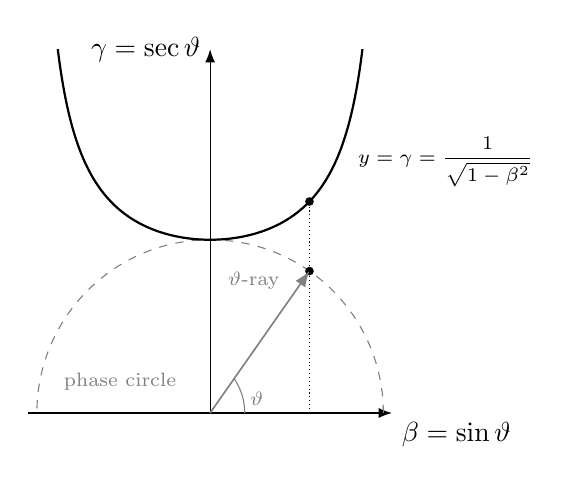
\begin{tikzpicture}[scale=2.2, >=Latex]
  % общие параметры
  \def\ymax{2.1}
  \def\th{35} % пример угла
  \pgfmathsetmacro{\bet}{sin(\th)}   % β = sin θ
  \pgfmathsetmacro{\co}{cos(\th)}    % cos θ
  \pgfmathsetmacro{\ga}{1/\co}       % γ = sec θ

  % оси (вне clip, чтобы надписи не резались)
  \draw[->] (-1.05,0) -- (1.05,0) node[below right] {$\beta=\sin\vartheta$};
  \draw[->] (0,0) -- (0,\ymax) node[left] {$\gamma=\sec\vartheta$};

  \begin{scope}
    \clip (-1.05,0) rectangle (1.95,\ymax);

    \draw[gray,dashed] (0,0) circle (1);

    \draw[line width=0.8pt] plot[domain=-0.90:0.90, samples=240] (\x, {1/sqrt(1-\x*\x)});

    \draw[densely dotted] (\bet,0) -- (\bet,\ga);
    \fill (\bet,\co) circle (0.025);
    \fill (\bet,\ga) circle (0.025);
  \end{scope}

  \draw[gray,->,line width=0.6pt] (0,0) -- (\bet,\co) node[pos=0.8, above left] {\scriptsize $\vartheta$-ray};
  \draw[gray] (0.20,0) arc[start angle=0, end angle=\th, radius=\th/100];
  \node[gray] at (0.27,0.08) {\scriptsize $\vartheta$};

  \node[gray] at (-0.52,0.18) {\scriptsize phase circle};
  \node at (1.36,1.45) {\scriptsize $y=\gamma=\dfrac{1}{\sqrt{1-\beta^{2}}}$};
\end{tikzpicture}
\caption{Phase circle vs. Lorentz hyperbola at common $\beta=\sin\vartheta$. Vertical mapping at fixed $\beta$ illustrates the Gudermann bridge: $\gamma=\sec\vartheta=\cosh\eta$.}
\label{fig:circle-hyperbola-gd}
\end{figure}
\FloatBarrier

%5 ===================================================================

\section{Phase space}

We represent a flow state on a quaternionic \emph{complex slice}
$\mathbb C_{\mathbf u}:=\mathrm{Span}\{1,\mathbf u\}\subset\mathbb H$,
where $\mathbf u\in S^2$ is the unit spatial direction selected by the observer’s split.
The unit rotor on this slice is
\[
\widehat q(\vartheta,\mathbf u):=\cos\vartheta+\mathbf u\,\sin\vartheta\in S^3\simeq SU(2),
\]
and, under the calibration $\|\boldsymbol\chi\|\equiv \clight$ (cf.\ §\ref{sec:calibration-c}),
we parameterize the flow vector as
\begin{equation}
\boldsymbol\chi(\vartheta,\mathbf u)=\clight\,\widehat q(\vartheta,\mathbf u)
=\clight\bigl(\cos\vartheta+\mathbf u\,\sin\vartheta\bigr).
\label{eq:phase-rotor-chi}
\end{equation}

\paragraph{Phase-rate projections (observer $A$).}\label{sec:phase-rates}
Given an observer $A$ with split $(\mathbf e_t^A,S^A)$ and
observer–object angle $\vartheta_{|\!A}$ (see \S\ref{sec:minkowski-derivation}),
the phase-rate components with respect to $A$ are
\begin{equation}
\tilde X^0_{|\!A}:=\frac{dx^0_{|\!A}}{d\chi}
=\clight\,\cos\vartheta_{|\!A},\qquad
\tilde{\mathbf X}_{|\!A}:=\frac{d\mathbf x_{|\!A}}{d\chi}
=\clight\,\sin\vartheta_{|\!A}\,\mathbf u_{|\!A},
\label{eq:phase-rates}
\end{equation}
where $\mathbf u_{|\!A}:=P_{S^A}\widehat{\mathbf F}/\|P_{S^A}\widehat{\mathbf F}\|\in S^A$ is the unit spatial
direction as seen by $A$ and $\widehat{\mathbf F}:=\boldsymbol\chi/\|\boldsymbol\chi\|$.

These rates satisfy the identity
\begin{equation}
\Bigl(\frac{ds}{d\chi}\Bigr)^2
=\bigl(\tilde X^0_{|\!A}\bigr)^2-\bigl\|\tilde{\mathbf X}_{|\!A}\bigr\|^2
=\clight^2\bigl(1-\sin^2\vartheta_{|\!A}\bigr)
=\clight^2\cos^2\vartheta_{|\!A}.
\label{eq:phase-budget-identity}
\end{equation}
which, in the SR simplification ($\zeta=\phi=0$ and $dt_A:=d\chi$), is just the operational split
of the fixed budget $\clight$ into temporal/spatial projections.

\paragraph{Phase-to-observable map (integral form).}
For any chart $x^i$ adapted to $A$ we have the integral transform
\begin{equation}
x^i(\chi)=x^i(\chi_0)+\int_{\chi_0}^{\chi}\tilde X^i_{|\!A}(u)\,du,
\qquad i=0,1,2,3,
\label{eq:phase-integral-map}
\end{equation}
with $\tilde X^0_{|\!A}$ and $\tilde{\mathbf X}_{|\!A}$ from \eqref{eq:phase-rates}. In the SR sector
this becomes
\(
t_A(\chi)=t_A(\chi_0)+\int_{\chi_0}^{\chi} du
\)
and
\(
\mathbf x_{|\!A}(\chi)=\mathbf x_{|\!A}(\chi_0)
+\int_{\chi_0}^{\chi}\clight\,\sin\vartheta_{|\!A}(u)\,\mathbf u_{|\!A}(u)\,du.
\)

\paragraph{Intrinsic vs.\ directional factors.}
The intrinsic second-moment angle $\zeta$ (\S\ref{sec:intrinsic-angle}) enters the body’s own
rate via $d\tau_B/d\chi=\cos\zeta$, while \eqref{eq:phase-rates} is purely directional and built
from the observer’s split. Outside the SR sector the intrinsic interval is
$ds_B^2=\clight^2\cos^2\zeta\,d\chi^2-d\boldsymbol\ell^{\!\top}\mathbf C_B\,d\boldsymbol\ell$,
and \eqref{eq:phase-integral-map} remains valid as a kinematic reconstruction of observables from
phase rates.

%6 ===================================================================
\section{Objects: operational catalogue and inference}
\label{sec:objects-catalogue}

\paragraph{Scope.} This section is a look-up summary. The physics and proofs live in
\S\ref{sec:body}, \S\ref{sec:intrinsic-angle}, \S\ref{sec:calibration-c}, and \S\ref{sec:phase-deriv}.

\subsection*{Canonical cases}
\begin{enumerate}
\item \textbf{Photon (vacuum).} \(\,T_B=0,\ d\tau_B=0,\ \|d\boldsymbol\ell\|/d\chi=\clight\) (Def.~\eqref{eq:calib-null}).
\item \textbf{Massive isotropic body.} \(\,\mathbf C_B=\frac{\sin^2\zeta}{3}\mathbf I,\quad
d\tau_B=\cos\zeta\,d\chi,\quad ds_B^2=\clight^2\cos^2\zeta\,d\chi^2-\frac{\sin^2\zeta}{3}\|d\boldsymbol\ell\|^2.\)
\item \textbf{Anisotropic body.} \(\,\mathbf C_B=\sum_{i=1}^3 \lambda_i\,\hat{\mathbf e}_i\otimes\hat{\mathbf e}_i,\ 
\lambda_i\ge0,\ \sum_i\lambda_i=\sin^2\zeta.\) Pullbacks along \(\hat{\mathbf e}_i\) probe \(\lambda_i\).
\item \textbf{Effective medium (\(\zeta\) only).} \(\,d\tau/dt=\cos\zeta,\ n(\zeta)=\sec\zeta\) (cf.\ \S\ref{ch:optics}).
\end{enumerate}

\subsection*{Parameter inference}
\begin{itemize}
\item \emph{Rate split at rest.} With \(\vartheta=0,\ \phi=0\): \(\cos\zeta=\bigl(d\tau_B/dt\bigr)_{\text{meas}}\).
\item \emph{Directional pullbacks.} Measure \(ds_B^2\) for small \(d\boldsymbol\ell\) along several lab directions;
fit the quadratic form \(q_B=d\boldsymbol\ell^\top\mathbf C_B\,d\boldsymbol\ell\Rightarrow\) eigenpairs \((\lambda_i,\hat{\mathbf e}_i)\).
\item \emph{Factorization with gravity/kinematics.} Use \(d\tau/dt=\cos\zeta\cos\phi\cos\vartheta\) to separate
\(\phi\) (clock angle) from \(\zeta\) via e.g.\ static vs moving protocols (see \S\ref{ch:optics}).
\end{itemize}

\subsection*{Ensemble composition}
For streamlets \(a\) with weights \(w_a\): \(T_B=\sum_a w_a\cos^2\Theta_a,\ 
\mathbf C_B=\sum_a w_a\sin^2\Theta_a\,\mathbf u_a\otimes\mathbf u_a\) (Eq.\ \eqref{eq:TB-CB}).

\subsection*{Non-collinear boosts}
Composition induces a spatial Wigner rotation on orientations without altering the scalar rate factorization;
see \S\ref{subsec:wigner}, \S\ref{subsec:thomas}.


%7 ===================================================================

\section{\texorpdfstring{Phase-derivative view}{Phase-derivative view}}
\label{sec:phase-deriv}

\noindent\textit{Scope.} This section repackages core identities in the language of
\emph{phase derivatives}, using only notions already introduced
(\S\ref{sec:calibration-c}–\ref{sec:minkowski-derivation}). No new kinematics is postulated.

\paragraph{Notation recap (from \S\ref{sec:phase-rates}).}
Phase–rate components for an observer $A$ are
\begin{equation}
\tilde X^0_{|\!A}=\frac{dx^0_{|\!A}}{d\chi}=\clight\,\cos\vartheta_{|\!A},\qquad
\tilde{\mathbf X}_{|\!A}=\frac{d\mathbf x_{|\!A}}{d\chi}
=\clight\,\sin\vartheta_{|\!A}\,\mathbf u_{|\!A},
\tag{\ref{eq:phase-rates}}
\end{equation}
and obey the identity
\begin{equation}
\Bigl(\frac{ds}{d\chi}\Bigr)^2
=\bigl(\tilde X^0_{|\!A}\bigr)^2-\bigl\|\tilde{\mathbf X}_{|\!A}\bigr\|^2
=\clight^2\bigl(1-\sin^2\vartheta_{|\!A}\bigr)
=\clight^2\cos^2\vartheta_{|\!A}.
\tag{\ref{eq:phase-budget-identity}}
\end{equation}
A change of parameter $\chi\mapsto\tau$ acts by the Jacobian $\mathcal J:=\dfrac{d\chi}{d\tau}$:
\begin{equation}
\dot X^i=\frac{d x^i}{d\tau}=\mathcal J\,\tilde X^i,\qquad
\dot{X}\equiv d/d\tau,\quad \tilde{X}\equiv d/d\chi.
\label{eq:param-change}
\end{equation}

\subsection{Minkowski–phase equality of invariants}
\label{subsec:phase-minkowski-equality}

\textbf{Theorem.} For any worldline segment and any observer $A$,
\begin{equation}
\boxed{\ \tilde H \;=\; \dot S\ },\qquad
\tilde H^2:=\bigl(\tilde X^0_{|\!A}\bigr)^2+\bigl\|\tilde{\mathbf X}_{|\!A}\bigr\|^2,\quad
\dot S^2:=\bigl(\dot X^0_{|\!A}\bigr)^2-\bigl\|\dot{\mathbf X}_{|\!A}\bigr\|^2 .
\label{eq:phase-minkowski-equality}
\end{equation}

\emph{Proof.} By \eqref{eq:param-change},
$\dot X^i=\mathcal J\,\tilde X^i$, hence
\[
\dot S^2=(\mathcal J\tilde X^0)^2-\|\mathcal J\tilde{\mathbf X}\|^2
=\mathcal J^2\!\left(\tilde X^0{}^2-\|\tilde{\mathbf X}\|^2\right)
=\mathcal J^2\Bigl(\frac{ds}{d\chi}\Bigr)^2
=\Bigl(\frac{ds}{d\tau}\Bigr)^2.
\]
At the same time,
$\tilde H^2=\tilde X^0{}^2+\|\tilde{\mathbf X}\|^2
=\clight^2$ in the SR gauge (\S\ref{subsec-1-5-sr-simplification}),
and $ds/d\tau=\clight$ by the operational split
$\cos\vartheta=d\tau/dt$, $\sin\vartheta=\|\mathbf v\|/\clight$ (\S\ref{sec:operational-phase}).
Therefore $\tilde H=\dot S=\clight$. $\square$

\paragraph{Reading.} In words: the Euclidean norm of the phase–rate vector equals the Minkowski
norm of the observable rate vector. The equality \eqref{eq:phase-minkowski-equality} is the
derivative form of “the same budget seen in two parametrizations”.

\subsection{Photon time: null interval and phase parameter}
\label{subsec:photon-phase-time}

For a lightlike flow in vacuum, the body’s intrinsic quadratic form gives
$ds_B^2=0$ (\S\ref{sec:calibration-c}), hence the body-level proper increment vanishes:
\begin{equation}
\boxed{\ d\tau_B=0\quad\text{(null flow, vacuum)}\ }.
\label{eq:photon-null}
\end{equation}
Nevertheless the phase parameter $\chi$ advances and serves as an affine parameter along
the ray. With the calibration \eqref{eq:calib-null} we have
\begin{equation}
\frac{\|d\boldsymbol\ell\|}{d\chi}=\clight,\qquad
\Rightarrow\quad \chi=\text{(cycle counter)}.
\label{eq:photon-affine}
\end{equation}

Under the convention $\Phi=\omega\,\chi$, one cycle corresponds to $\Delta\chi=2\pi/\omega$, so $\chi$ counts
wavefronts affinely while the intrinsic metric remains null ($d\tau_B=0$).


At unit frequency, $\nu:=d\chi/d\tau=1$, the phase equals the proper-time parameter used as an
affine label of wavefronts; no contradiction with \eqref{eq:photon-null} arises because
$\tau$ here is a \emph{chosen} parameter for counting cycles, while the intrinsic
metric length remains null.

% --- PATCH: insert after § Mapping to SR (before or after the correspondences table) ---

\subsection{Relativistic Doppler as a phase–kinematic theorem}\label{sec:doppler-core}

We derive the Doppler law purely from the phase split, without hyperbolic parametrization or dynamics.

\paragraph{Setup.}
Define frequency as the phase growth rate in proper time,
\(
\nu:=d\chi/d\tau
\),
and consider two successive wavefronts separated by the same phase increment
\(
\Delta\chi
\)
for the source and the observer. Then
\begin{equation}
\frac{\nu_{\mathrm{obs}}}{\nu_{\mathrm{src}}}
=\frac{d\chi/d\tau_{\mathrm{obs}}}{d\chi/d\tau_{\mathrm{src}}}
=\frac{d\tau_{\mathrm{src}}}{d\tau_{\mathrm{obs}}}.
\label{eq:doppler-core-master}
\end{equation}

In the SR sector (\(\zeta=\phi=0\)) the observer at rest has \(d\tau_{\mathrm{obs}}=dt_{\mathrm{obs}}\),
and for the (possibly moving) source \(dt_{\mathrm{src}}=\gamma\,d\tau_{\mathrm{src}}\) with
\(\gamma=\sec\vartheta\), \(\beta=\sin\vartheta\).

\paragraph{Longitudinal case.}
During the emission interval \(dt_{\mathrm{src}}=\gamma\,d\tau_{\mathrm{src}}\) (measured in the
observer’s lab chart) the source shifts by \(\pm \beta c\,dt_{\mathrm{src}}\) along the line of sight
(“\(+\)” receding, “\(-\)” approaching). The reception interval is the emission interval plus the
change in light flight time:
\[
dt_{\mathrm{obs}}
= dt_{\mathrm{src}} \,\bigl(1\pm \beta\bigr)
= \gamma\,d\tau_{\mathrm{src}} \,\bigl(1\pm \beta\bigr).
\]
With \eqref{eq:doppler-core-master} and \(d\tau_{\mathrm{obs}}=dt_{\mathrm{obs}}\) this gives the Doppler factor
\begin{equation}
\boxed{\ \frac{\nu_{\mathrm{obs}}}{\nu_{\mathrm{src}}}
=\frac{1}{\gamma(1\pm\beta)}\ }
=\sqrt{\frac{1\mp\beta}{1\pm\beta}}
=\sec\vartheta\,(1\mp\sin\vartheta)
=e^{\mp\eta},
\label{eq:doppler-core-long}
\end{equation}
where the equivalent forms use \(\beta=\sin\vartheta\), \(\gamma=\sec\vartheta\), and the Gudermann bridge \eqref{eq:gudermann}.

\paragraph{Transverse case.}
For \(\varphi=90^\circ\) (emission orthogonal to the relative velocity in the observer’s frame),
the geometric flight-time correction vanishes, hence
\begin{equation}
\boxed{\ \frac{\nu_{\mathrm{obs}}}{\nu_{\mathrm{src}}}=\frac{1}{\gamma}=\cos\vartheta\ }.
\label{eq:doppler-core-trans}
\end{equation}

\paragraph{General line-of-sight angle.}
Let \(\varphi\) be the angle between the source velocity and the line of sight in the observer’s frame.
Only the LOS component \(\beta\cos\varphi\) changes the flight time; repeating the above,
\begin{equation}
\boxed{\ \frac{\nu_{\mathrm{obs}}}{\nu_{\mathrm{src}}}
=\frac{1}{\gamma\,(1-\beta\cos\varphi)}
\ =\ \gamma\,(1-\beta\cos\varphi)^{-1}\ }.
\label{eq:doppler-core-los}
\end{equation}
Equivalently, in phase variables,
\(\nu_{\mathrm{obs}}/\nu_{\mathrm{src}}=\sec\vartheta\,\bigl(1-\sin\vartheta\cos\varphi\bigr)^{-1}\).

\paragraph{Corollary (with intrinsic/gravitational tilts).}
Outside the pure SR sector, the total redshift factorizes:
\[
1+z_{\rm tot}
=\frac{\nu_{\mathrm{src}}}{\nu_{\mathrm{obs}}}
=\underbrace{\gamma(1-\beta\cos\varphi)}_{\text{kinematic}}
\,\times\,
\underbrace{\frac{\cos\zeta_{\rm obs}\cos\phi_{\rm obs}}{\cos\zeta_{\rm src}\cos\phi_{\rm src}}}_{\text{intrinsic \& gravitational}},
\]
which reproduces \eqref{eq:z-factorization} upon identifying the kinematic part with
\eqref{eq:doppler-core-los}.

\paragraph{Infinitesimal form (longitudinal).}
Taking the differential of $\ln(\nu_{\mathrm{obs}}/\nu_{\mathrm{src}})$,
\begin{equation}
\boxed{\ d\ln\frac{\nu_{\mathrm{obs}}}{\nu_{\mathrm{src}}}
= \mp\,d\eta
= \mp\,\sec\vartheta\,d\vartheta
= \mp\,\gamma^{2}\,d\beta\ },
\label{eq:doppler-inf-long}
\end{equation}
with the upper sign for receding (“$+$” in \eqref{eq:doppler-core-long}) and lower for approaching.
Equation \eqref{eq:doppler-inf-long} is the \emph{phase–derivative} Doppler law.

\paragraph{Transverse case.}
For $\varphi=90^\circ$ in the observer’s frame the flight-time correction vanishes,
so $\nu_{\mathrm{obs}}/\nu_{\mathrm{src}}=1/\gamma$ and
\begin{equation}
d\ln\frac{\nu_{\mathrm{obs}}}{\nu_{\mathrm{src}}}=-\,d\ln\gamma=-\beta\gamma^2\,d\beta.
\label{eq:doppler-inf-trans}
\end{equation}

\paragraph{General LOS angle (fixed geometry).}
If $\varphi$ is the angle between the velocity and the line of sight in the observer’s frame and
$d\varphi=0$, then from
$\nu_{\mathrm{obs}}/\nu_{\mathrm{src}}=1/\bigl[\gamma(1-\beta\cos\varphi)\bigr]$ one gets
\begin{equation}
d\ln\frac{\nu_{\mathrm{obs}}}{\nu_{\mathrm{src}}}
=-\Bigl[\beta\gamma^2-\frac{\cos\varphi}{1-\beta\cos\varphi}\Bigr]\,d\beta
\ =\ -\,d\eta\ \ \text{when }\ \varphi=0,\pi .
\label{eq:doppler-inf-los}
\end{equation}

\medskip
Together, \eqref{eq:phase-minkowski-equality}, \eqref{eq:photon-null}–\eqref{eq:photon-affine}, and
\eqref{eq:doppler-inf-long}–\eqref{eq:doppler-inf-los} show how \emph{phase derivatives} encode:
(i) equality of observable and phase invariants;
(ii) the null nature of photon proper time with $\chi$ as an affine counter;
(iii) the Doppler law, both finite and in instantaneous differential form.

%8 ===================================================================

\section{Unified temporal effects in phase space}
\label{ch:optics}

We factor all time-related effects through a single phase tilt structure.
Let the intrinsic (\(\zeta\)), gravitational (\(\phi\)), and kinematic (\(\vartheta\)) angles be independent contributors to the phase tilt at a point.
Define the local \emph{time-rate factor}
\begin{equation}
\label{eq:time-rate-factor}
\frac{d\tau}{dt}
\;=\;
\cos\zeta\;\cos\phi\;\cos\vartheta,
\qquad
n_{\rm tot}\;:=\;\sec\zeta\;\sec\phi\;\sec\vartheta,
\end{equation}
where \(n_{\rm tot}\) plays the role of an effective (phase) refractive index for light propagation.
Accordingly, the coordinate light-travel time along a spatial curve \(\Gamma\) is
\begin{equation}
\label{eq:optical-length}
t_\Gamma \;=\; \frac{1}{\clight}\int_\Gamma n_{\rm tot}\,ds.
\end{equation}

\paragraph{Lemma (Unified time-rate).}
In the unimetry phase representation, the proper-to-lab time rate and the optical length factorize as in \eqref{eq:time-rate-factor}–\eqref{eq:optical-length}.
Setting any subset of angles to zero recovers the corresponding standard effects:
\begin{itemize}\itemsep4pt
  \item \textbf{Special relativity (vacuum SR):} \(\zeta=0,\ \phi=0\Rightarrow d\tau/dt=\cos\vartheta=1/\gamma\) (kinematic time dilation).
  \item \textbf{Gravitational clocks (static weak field):} \(\zeta=0,\ \vartheta=0\Rightarrow d\tau/dt=\cos\phi\) (gravitational redshift/clock rate); calibration of \(\phi\) reproduces the usual \(\sqrt{g_{00}}\).
  \item \textbf{Shapiro delay (gravitational contribution to TOF):} with \(\zeta=0,\ \vartheta=0\), \eqref{eq:optical-length} yields \(t_\Gamma=(1/\clight)\int \sec\phi\,ds\); the excess over \(\int ds/\clight\) is the Shapiro time delay.
  \item \textbf{Intrinsic/evolutionary tilt:} \(\phi=0,\ \vartheta=0\Rightarrow d\tau/dt=\cos\zeta,\ n_{\rm tot}=\sec\zeta\) (useful as a time gauge in cosmological/effective-medium contexts).
\end{itemize}

\paragraph{Remarks.}
(i) The factorization in \eqref{eq:time-rate-factor} is the phase-space counterpart of composing independent tilts; it preserves the conserved Minkowski norm once time is reparameterized by \(\tau\).
(ii) For vacuum SR we simply set \(\zeta=0\) and work with \(\vartheta\); for pure gravitational timing we set \(\vartheta=0\) and use \(\phi\).
(iii) Non-collinear boost composition acts on \(\vartheta\) via quaternionic rotors and induces a Wigner/Thomas residual \emph{spatial} rotation without altering \eqref{eq:time-rate-factor}.

%9 ===================================================================

\section{\texorpdfstring{Gravity as a phase rotation: local tetrads and clock angle}{Gravity as a phase rotation}}

On a curved background $(\mathcal M,g)$ we work with orthonormal tetrads $e_a{}^\mu$ such that $g_{\mu\nu}e_a{}^\mu e_b{}^\nu=\eta_{ab}$ and take the observer's time leg to be $e_0{}^\mu$. 
We apply the gravitational (clock) angle $\phi$ as
\begin{equation}
\cos\phi\ :=\ e^0{}_\mu\,u^\mu\ =\ \frac{d\tau_{\rm stat}}{dt}\ =\ \sqrt{-g_{00}}\qquad\text{(stationary case)}.
\label{eq:clock-angle}
\end{equation}

Kinematics remains encoded by the phase angle $\vartheta$ in the slice $\mathbb C_{\mathbf u}$, with
$\cos\vartheta=d\tau/d\tau_{\rm stat}$. 
Therefore the proper time factorizes as
\begin{equation}
d\tau\ =\ dt\,\cos\phi\,\cos\vartheta,\qquad 
d\mathbf x\ =\ c\,dt\,\sin\vartheta\,\mathbf u,
\label{eq:tau-factorization}
\end{equation}
and the total redshift factorizes into kinematic and gravitational parts:
\begin{equation}
1+z_{\rm tot}\ =\ \frac{\cos\vartheta_{\rm em}}{\cos\vartheta_{\rm obs}}\ \times\ 
\frac{\cos\phi(x_{\rm em})}{\cos\phi(x_{\rm obs})}.
\label{eq:z-factorization}
\end{equation}

For static emitter/observer ($\vartheta_{\rm em}=\vartheta_{\rm obs}=0$) one recovers the standard gravitational redshift 
$1+z_g=\sqrt{\frac{-g_{00}(x_{\rm obs})}{-g_{00}(x_{\rm em})}}$.
In the weak-field limit $g_{00}\simeq-(1+2\Phi/ \clight^2)$ this gives $z_g\simeq(\Phi_{\rm obs}-\Phi_{\rm em})/c^2$.

\paragraph{Beyond static fields.}
In a $3\!+\!1$ split $ds^2=-N^2 \clight^2 dt^2 + h_{ij}(dx^i+N^i dt)(dx^j+N^j dt)$ one may identify $\cos\phi:=N$ in the observer's tetrad, which keeps \eqref{eq:tau-factorization}–\eqref{eq:z-factorization} coordinate-agnostic.
Uniform acceleration (Rindler) accumulates phase according to $d\vartheta=\kappa\,dt$ inside the local slice, consistently reproducing accelerated-frame kinematics when combined with the clock angle $\phi$.

%9 ===================================================================

\section{Discussion}

The phase-space reformulation of special relativity presented in this work provides an original and conceptually unifying framework, recasting all standard kinematic effects as geometric projections and rotations within a Euclidean (as opposed to pseudo-Euclidean) phase space structured by the algebra of quaternions. This approach enables closed-form derivations of time dilation, Lorentz contraction, all Doppler effects, and the composition of boosts—including the emergence of Wigner and Thomas rotations—as pure consequences of phase kinematics and composition rules for rotors. Notably, the speed of light appears not as a postulate but as a derived invariant: the magnitude of the calibrated flow.

One of the main strengths of the unimetry approach is its ability to coherently and transparently separate intrinsic, gravitational, and kinematic effects through the introduction of independent angular parameters. This structural modularity allows for clear generalizations beyond the regime of special relativity (SR). The use of quaternionic algebra naturally incorporates the noncommutative composition of boosts (and hence Wigner rotation), and the direct operational mapping from phase parameters to observable quantities avoids the hyperbolic constructs and nested root expressions traditional to the Lorentzian metric, potentially offering both conceptual and computational simplifications.

The revisit of the kinematical foundations of relativity within a Euclidean metric is reminiscent of various efforts to find deeper group-theoretic or geometric underpinnings for known physics, such as the reinterpretation of quantum spinors, twistors, or the generalized use of Clifford and quaternionic structures. 

Despite these advantages, there are several limitations and open issues:
\begin{itemize}
    \item The present work, while offering a full reformulation of SR, leaves the dynamical aspects---especially those tied to gravitational fields and interactions---outside its direct scope. The approach to gravity as a phase tilt field is promising, but it will require a precise translation of Einsteinian field dynamics into the quaternionic, phase-based language.
    \item Similarly, the connection to quantum mechanics, though structurally motivated by the phase-space formulation and inherent links to phase and geometric quantization, remains undeveloped at the level of operator theory or Hilbert space structures. Concrete examples or models connecting unimetry directly to quantum phenomena would reinforce the physical scope and relevance of the approach.
    \item A key question for future study is the physical interpretability and experimental accessibility of the various angular parameters (intrinsic, gravitational, kinematic) in more complex, curved, or quantum-influenced scenarios.
    \item The mathematical tools used---particularly the phase decomposition and modularization---have strong implications for the construction of algorithms in numerical relativity and simulation of accelerated particle beams, but explicit comparisons with existing computational methods remain to be presented.
\end{itemize}


\section*{Outlook}

The unimetry framework developed here provides a versatile foundation for future theoretical developments in both relativity and quantum physics. The following directions emerge as particularly promising:
\begin{itemize}
    \item
    \textbf{Extension to General Relativity.} The modular phase decomposition is well suited for the introduction of curved metrics, potentially allowing gravitational redshift, time delay (Shapiro effect), and even curvature-driven precessions to be recast in the language of phase tilts and generalized rotors. Realizing Einstein's dynamics for gravitational fields in this formalism is a natural next step, especially via the local tetrad and clock angle structures already sketched.

    \item
    \textbf{Quantum Connections.} Given the central role of phase, rotors, and symmetry groups (notably the demonstration of Hopf fibration structure), the unimetry formalism can serve as a stepping stone toward a deeper unification between relativistic and quantum frameworks, possibly via geometric quantization or generalized qubit/Bloch-sphere analogues.

    \item
    \textbf{Physical and Experimental Applications.} The structure is already suited for reinterpretation and numerical simulation of phenomena involving non-collinear accelerations, such as in advanced particle beam physics or optical systems with phase media. This computational potential deserves further methodological and comparative exploration.

    \item
    \textbf{Generalizations and Group Theory.} The embedding of Lorentzian kinematics within a more general Euclidean group-theoretic framework (potentially encompassing de Sitter or conformal transformations) may suggest further extensions, including nontrivial topologies, higher dimensions, or self-dual (instanton-like) solutions.
\end{itemize}

In summary, by replacing the traditional spacetime paradigm with a geometric flow in phase space, unimetry opens avenues for new mathematical structures and connections among relativity, geometry, and quantum theory. Its broader success will depend on future progress in developing the gravitational and quantum sectors and on the demonstration of concrete computational and experimental advantages.




\appendix
\section{Equivalence to the classical Wigner rotation}
\label{app:1}

We sketch an intrinsic quaternionic proof that the unimetry expression for the Wigner rotation
coincides with the standard special-relativistic formula.

\paragraph{Step 1: product of two D-rotors.}
For $d_i=\cos\frac{\psi_i}{2}+\uhat_i\sin\frac{\psi_i}{2}$,
\begin{equation}
\label{eq:auto:45}
d_2 d_1
=(c_2c_1-s_2s_1\cos\theta)
+\Big(c_2s_1\uhat_1+s_2c_1\uhat_2+s_2s_1\,\uhat_2\times\uhat_1\Big),
\end{equation}
with $c_i=\cos(\psi_i/2)$, $s_i=\sin(\psi_i/2)$ and $\cos\theta=\uhat_2\!\cdot\!\uhat_1$.

\paragraph{Step 2: symmetric D--R factorization.}
Define $d_{12}$ by $d_{12}\,\mathbf e_t\, d_{12}=L_{12}\,\mathbf e_t\, L_{21}$ and set
$r_W=\bar d_{12}\,L_{12}=L_{21}\,\bar d_{12}$. Then $r_W$ fixes $\mathbf e_t$ and is a pure spatial
rotor, so $r_W=\cos\frac{\phi}{2}+\hat{\mathbf n}\sin\frac{\phi}{2}$ with
$\hat{\mathbf n}\parallel \uhat_2\times\uhat_1$. Matching scalar and bivector parts gives
\begin{equation}
\tan\frac{\phi}{2}=
\frac{s_1 s_2\,\sin\theta}{\,c_1 c_2+s_1 s_2\,\cos\theta\,}.
\label{eq:uni-phi}
\end{equation}

\paragraph{Step 3: map to rapidities.}
With the substitutions $\sin(\psi/2)\mapsto\sinh(\eta/2)$, $\cos(\psi/2)\mapsto\cosh(\eta/2)$,
$\tan(\psi/2)\mapsto\tanh(\eta/2)$ (where $\tanh\eta=\beta$, $\cosh\eta=\gamma$), \eqref{eq:uni-phi}
becomes the textbook Wigner angle:
\begin{equation}
\label{eq:auto:47}
\tan\frac{\phi}{2}
=\frac{\sinh\frac{\eta_1}{2}\,\sinh\frac{\eta_2}{2}\,\sin\theta}
{\cosh\frac{\eta_1}{2}\,\cosh\frac{\eta_2}{2}+\sinh\frac{\eta_1}{2}\,\sinh\frac{\eta_2}{2}\,\cos\theta},
\end{equation}
with axis along $\uhat_2\times\uhat_1$. This circular--hyperbolic correspondence is classical; cf.\ Gudermann~\cite{Gudermann1830}.

\end{document}
